\documentclass{beamer}
\usepackage[spanish]{babel}
\usepackage[utf8]{inputenc}
\usepackage{braket}
\usepackage{ragged2e,color,textcomp,multicol,geometry,cancel,etoolbox}
\usepackage{multirow}
%\usepackage[latin1]{inputenc} PARA MACs
\usepackage{bm} %letras griegas en negrita (uso: \bm{\alpha})
\newcommand{\vect}[1]{\boldsymbol{\mathbf{#1}}}
\title[]{Caracterización de la emisión en radio en cascadas atmosféricas iniciadas por
neutrinos tau de muy altas energías en detectores a gran altitud}

\author[USC. Curso 2021/22]{\textit{Trabajo de Fin de Máster}\vspace{5mm}\\\textit{Autor:} Sergio Cabana Freire\vspace{5mm}\\\textit{Tutor:} Jaime Álvarez Muñiz}
\date[Trabajo Fin de Máster]{}

\usetheme{Madrid} %Selección de Tema.

% Galería de temas: http://deic.uab.es/~iblanes/beamer_gallery/

\apptocmd{\frame}{}{\justifying}{}
\beamertemplatenavigationsymbolsempty
\AtBeginSection[]
{
	\begin{frame}
		\tableofcontents[currentsection]
	\end{frame}
}

\begin{document}
	\begin{frame}[plain, noframenumbering]
		\titlepage
		\vspace{-15mm}
		\begin{columns}
		\column{.5\textwidth}
		\begin{figure}[H]
		\centering
		
\includegraphics[width=.45\linewidth]{figures/USC}
		\end{figure}
		\column{.5\textwidth}
		\begin{center}
		\textit{Facultad de Física, USC}
		\vspace{5mm}\\
		20 de julio de 2022
		\end{center}
		\end{columns}
	\end{frame}
	
	\begin{frame}[plain, noframenumbering]{Contenidos}
		\tableofcontents
	\end{frame}
	\section{Introducción}
	\begin{frame}{Introducción}
		\begin{itemize}
			\item Descubrimientos recientes $\rightarrow$ Astronomía de Multi-mensajeros (EM, GW, neutrinos, rayos cósmicos, ...)
			\item Nuevas posibilidades de observación y estudio de fenómenos astrofísicos
		\end{itemize}
		\pause\begin{block}{\centering Neutrinos $\rightarrow$ Baja probabilidad de interacción}

		\begin{columns}
			\column{.45\textwidth}
			\centering
			$\bullet$Información directa desde las fuentes
			
			$\bullet$Propagación rectilínea, escasa pérdida de energía
			
			$\bullet$Acceso a regiones EM opacas
			\column{.45\textwidth}
			\centering
			$\bullet$Grandes dificultades para detección
			
			$\bullet$Escasos flujos a las mayores energías
			
			$\bullet$Detectores de gran exposición
		\end{columns}
		\end{block}
	\end{frame}
\begin{frame}{Introducción II}
		\begin{equation*}
		\text{Interacción hadrónica de rayos cósmicos}\left\{\begin{array}{l}\pi^0\rightarrow \gamma\gamma\\\pi^+\rightarrow \mu^+ \bm{\nu_\mu}\rightarrow e^+ \bm{\nu_e \overline{\nu}_\mu \nu_\mu}\\ \pi^-\rightarrow \mu^- \bm{\overline{\nu}_\mu}\rightarrow e^- \bm{\overline{\nu}_e \nu_\mu \overline{\nu}_\mu}\end{array}\right.\;.\label{ec11}
	\end{equation*}
	\pause\begin{equation*}
		\text{Flujo de neutrinos}\left\{\begin{array}{l}\text{Fuentes concretas}\left\{\begin{array}{l}\text{Galácticas}\\\text{Extragalácticas}\end{array}\right.\\\text{Flujos difusos}\end{array}\right.
	\end{equation*}

\begin{itemize}
	\item Información sobre producción de CR's (interacciones en fuentes) y sobre su propagación (medio intergaláctico)
\end{itemize}
\pause\begin{block}{\centering Posibilidad para detección}
	\centering \textit{Observación de radiación electromagnética en frecuencias $\mathrm{MHz-GHz}$ emitida en cascadas atmosféricas de partículas}
	\end{block}
\end{frame}
\begin{frame}{Introducción III}
	\begin{itemize}
		\item Objetivo: Detección de neutrinos tau interaccionando en el interior de la Tierra y generando cascadas atmosféricas hacia arriba. 
		\item Radiodetección $\rightarrow$ Monitorización de grandes áreas con detectores a gran altitud (BEACON, ANITA, PUEO). Posibilidad de emplear la Tierra como blanco de interacción.
	\end{itemize}
	\begin{figure}[H]
	\centering
	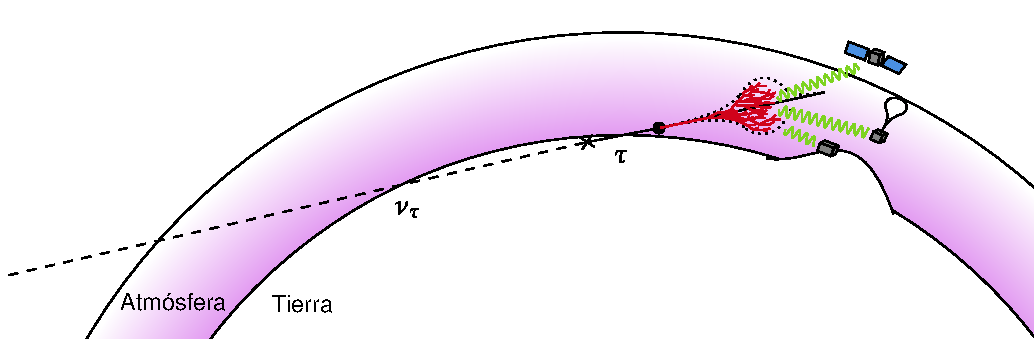
\includegraphics[width=1\linewidth]{figures/shower_up_v2}
	\end{figure}
\end{frame}
	\section{Cascadas atmosféricas}
	\begin{frame}{Cascadas atmosféricas}
		\begin{itemize}
			\item Detección indirecta de partículas de alta energía $\rightarrow$ Interacciones producen un nº elevado de partículas propagándose en la atmósfera (cascada), detección con diversas técnicas.
		\end{itemize}
			\begin{figure}[H]
				\centering
				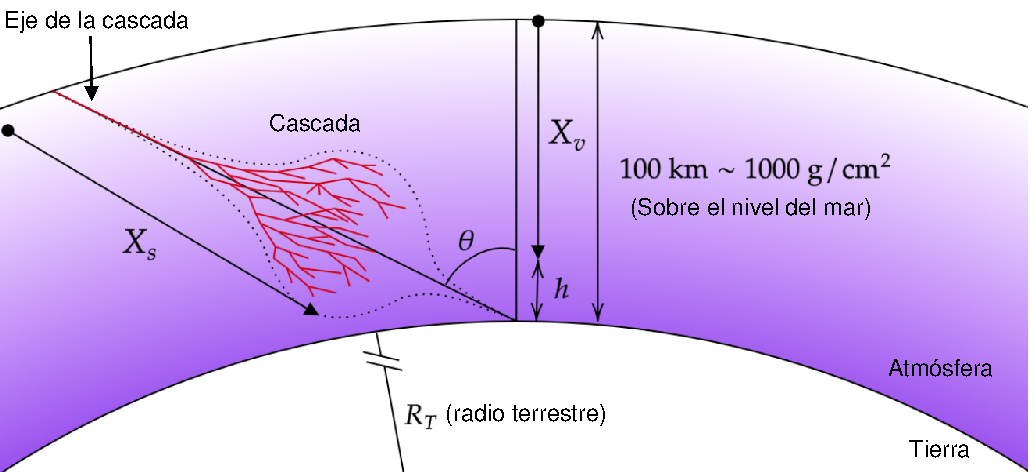
\includegraphics[width=.7\linewidth]{figures/cascadas/shower_params_v2}
			\end{figure}
		\begin{itemize}
			\item Atmósfera inhomogénea $\rightarrow$ Materia atravesada como magnitud clave. 
		\end{itemize}
	\end{frame}
\begin{frame}{Cascadas atmosféricas II}
		\begin{figure}[H]
			\centering
			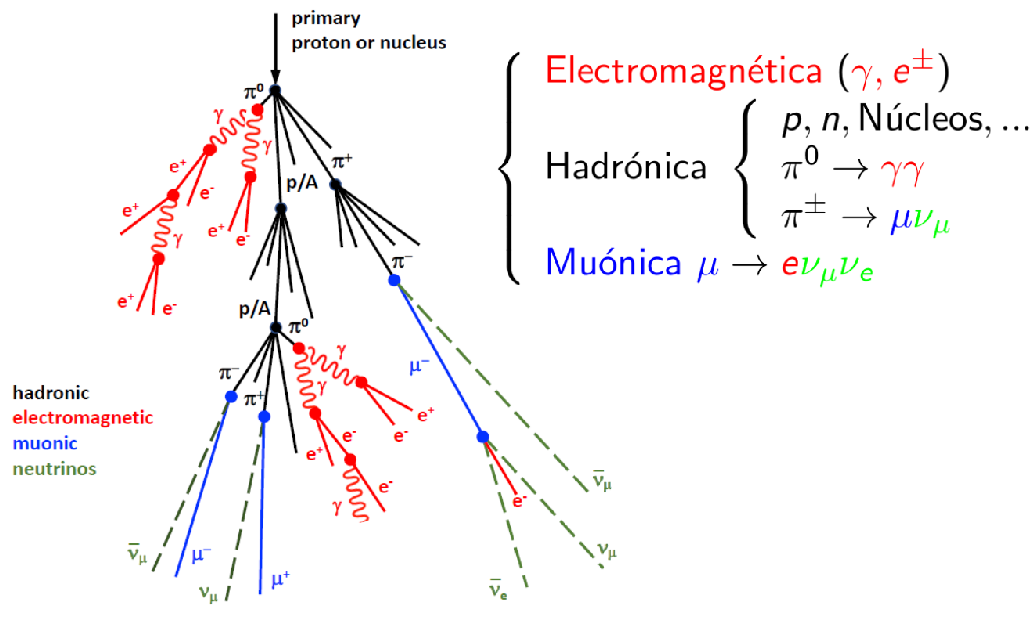
\includegraphics[width=.65\linewidth]{figures/EAS_sketch}
		\end{figure}
		\color{black}
		\begin{itemize}
		\item Desarrollo $\rightarrow$ Competición entre interacción ($\uparrow$ nº partículas) frente a desintegraciones.
	\end{itemize}
\pause\begin{block}{\centering Simulaciones con AIRES (v. 2.8.4a)}
	\centering Desarrollo de cascadas hacia arriba según ángulo cenital $\theta$, energía y naturaleza del primario. Comparación con cascadas hacia abajo.
\end{block}
\end{frame}

\begin{frame}{Ángulo cenital $\theta$}
	\begin{itemize}
		\item Primario protón de $1\,\mathrm{EeV}$ interaccionando a $5\,\mathrm{km}$ de altura.
	\end{itemize}
		\begin{figure}[H]
		\centering
		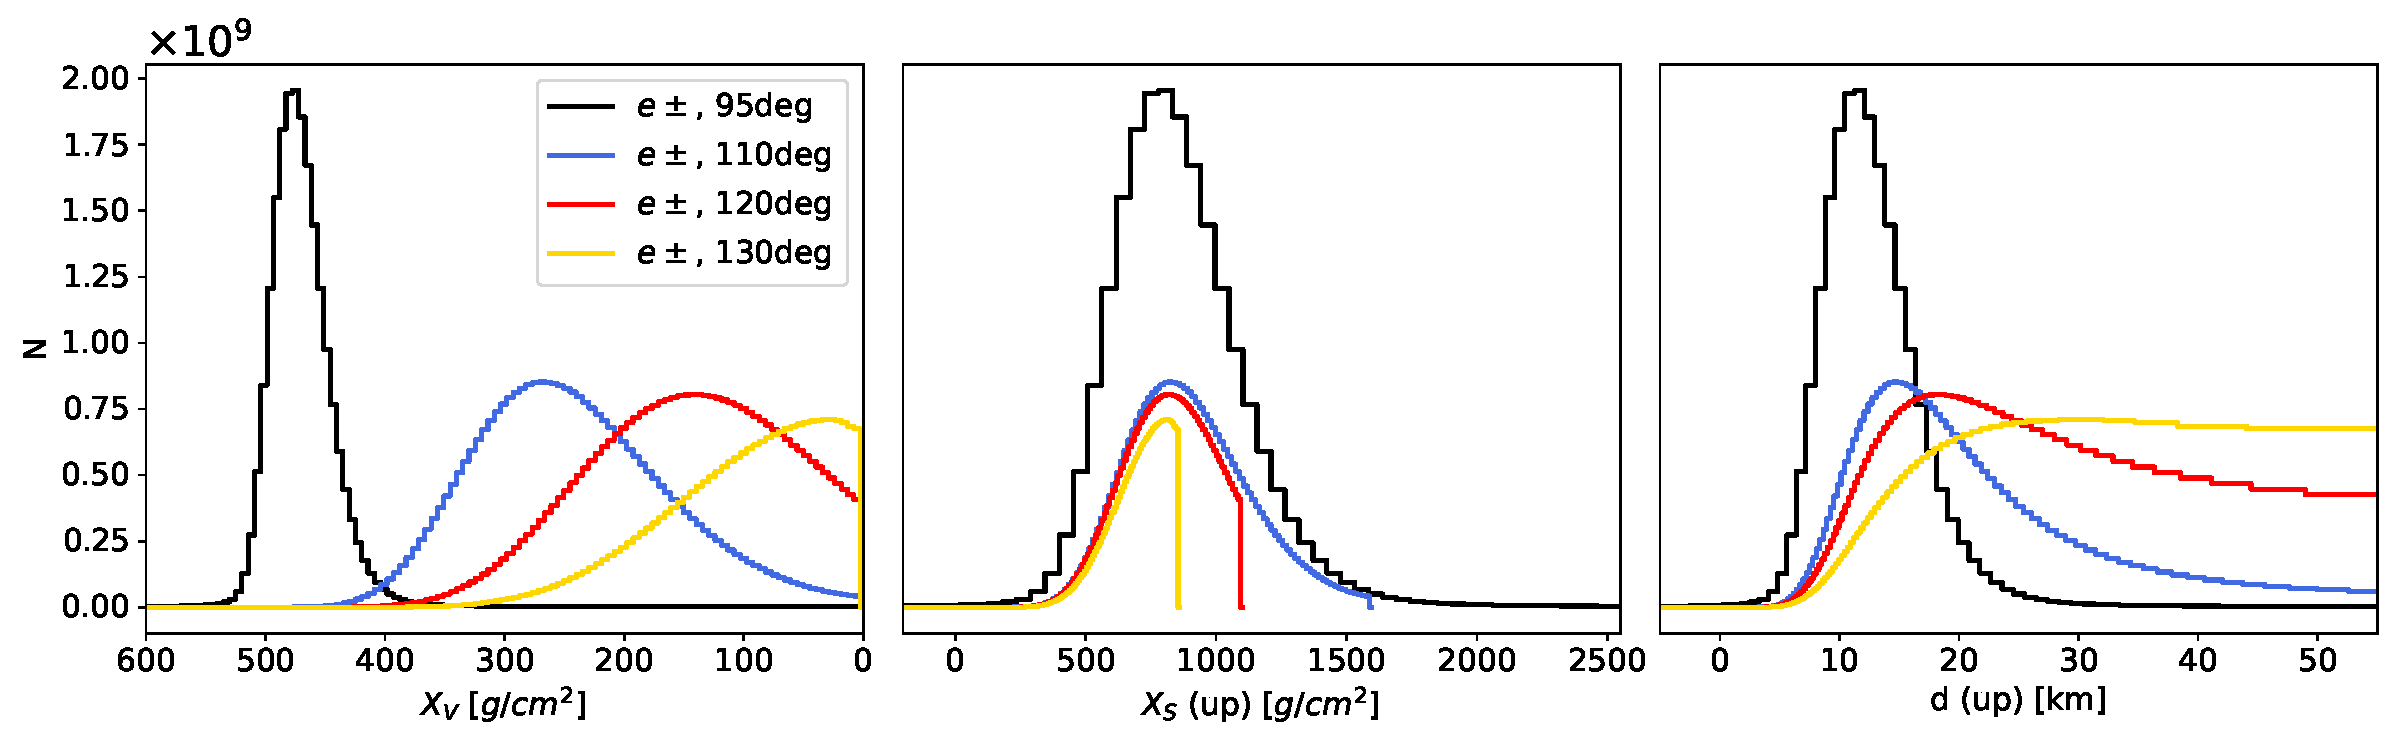
\includegraphics[width=.95\linewidth]{figures/cascadas/upgoing_p_1EeV_vardeg_5km_e_v2}
	\end{figure}
	\begin{figure}[H]
	\centering
	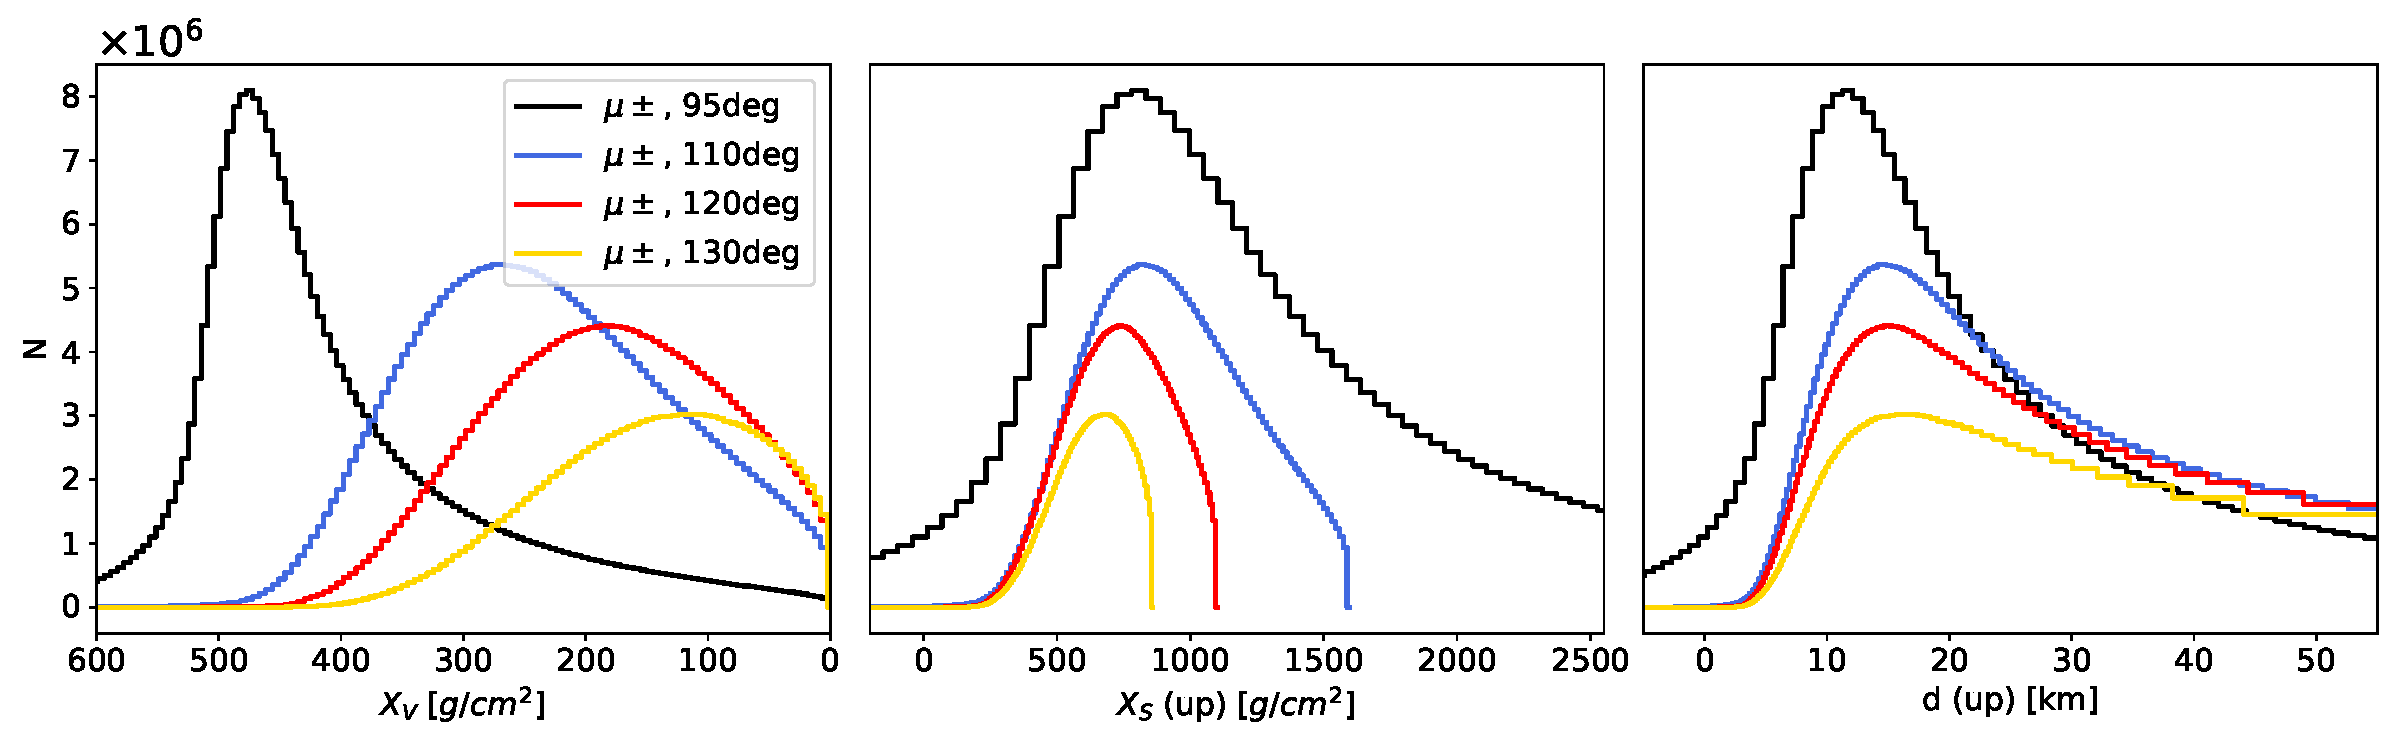
\includegraphics[width=.95\linewidth]{figures/cascadas/upgoing_p_1EeV_vardeg_5km_mu_v2}
\end{figure}
\end{frame}

\begin{frame}{Ángulo cenital $\theta$. Comentarios}
	\begin{itemize}
		\item El máximo nº de partículas decrece con el ángulo (cascadas más verticales) $\rightarrow$ Desarrollo en zonas menos densas.
		\item La posición del máximo de $e^\pm$ (EM) sólo depende de la materia atravesada.
		\item La posición del máximo de $\mu^\pm$ depende del ángulo $\rightarrow$ Efecto de desintegraciones en zonas menos densas.
		\item Al aumentar $\theta$, se necesita recorrer una mayor distancia para alcanzar el máximo del desarrollo.
	\end{itemize}
		\begin{figure}[H]
	\centering
	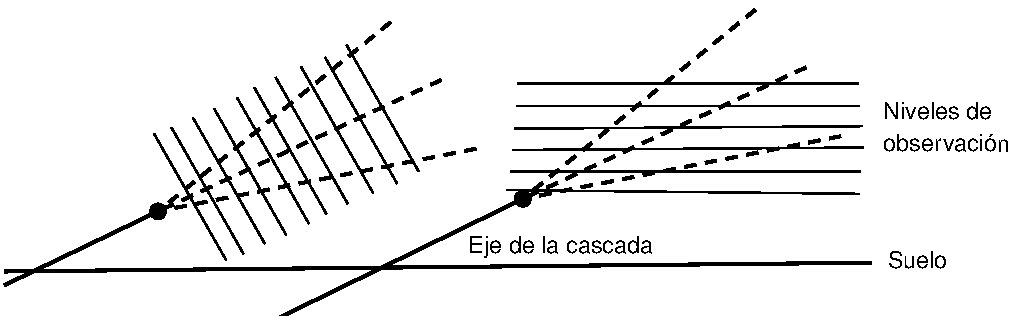
\includegraphics[width=.65\linewidth]{figures/cascadas/AIRES_planos_v2}
\end{figure}
\end{frame}
\begin{frame}{Energía del primario}
		\begin{itemize}
		\item Primario protón a $\theta = 95^\circ$ interaccionando a $5\,\mathrm{km}$ de altura.
	\end{itemize}
	\begin{figure}[H]
		\centering
		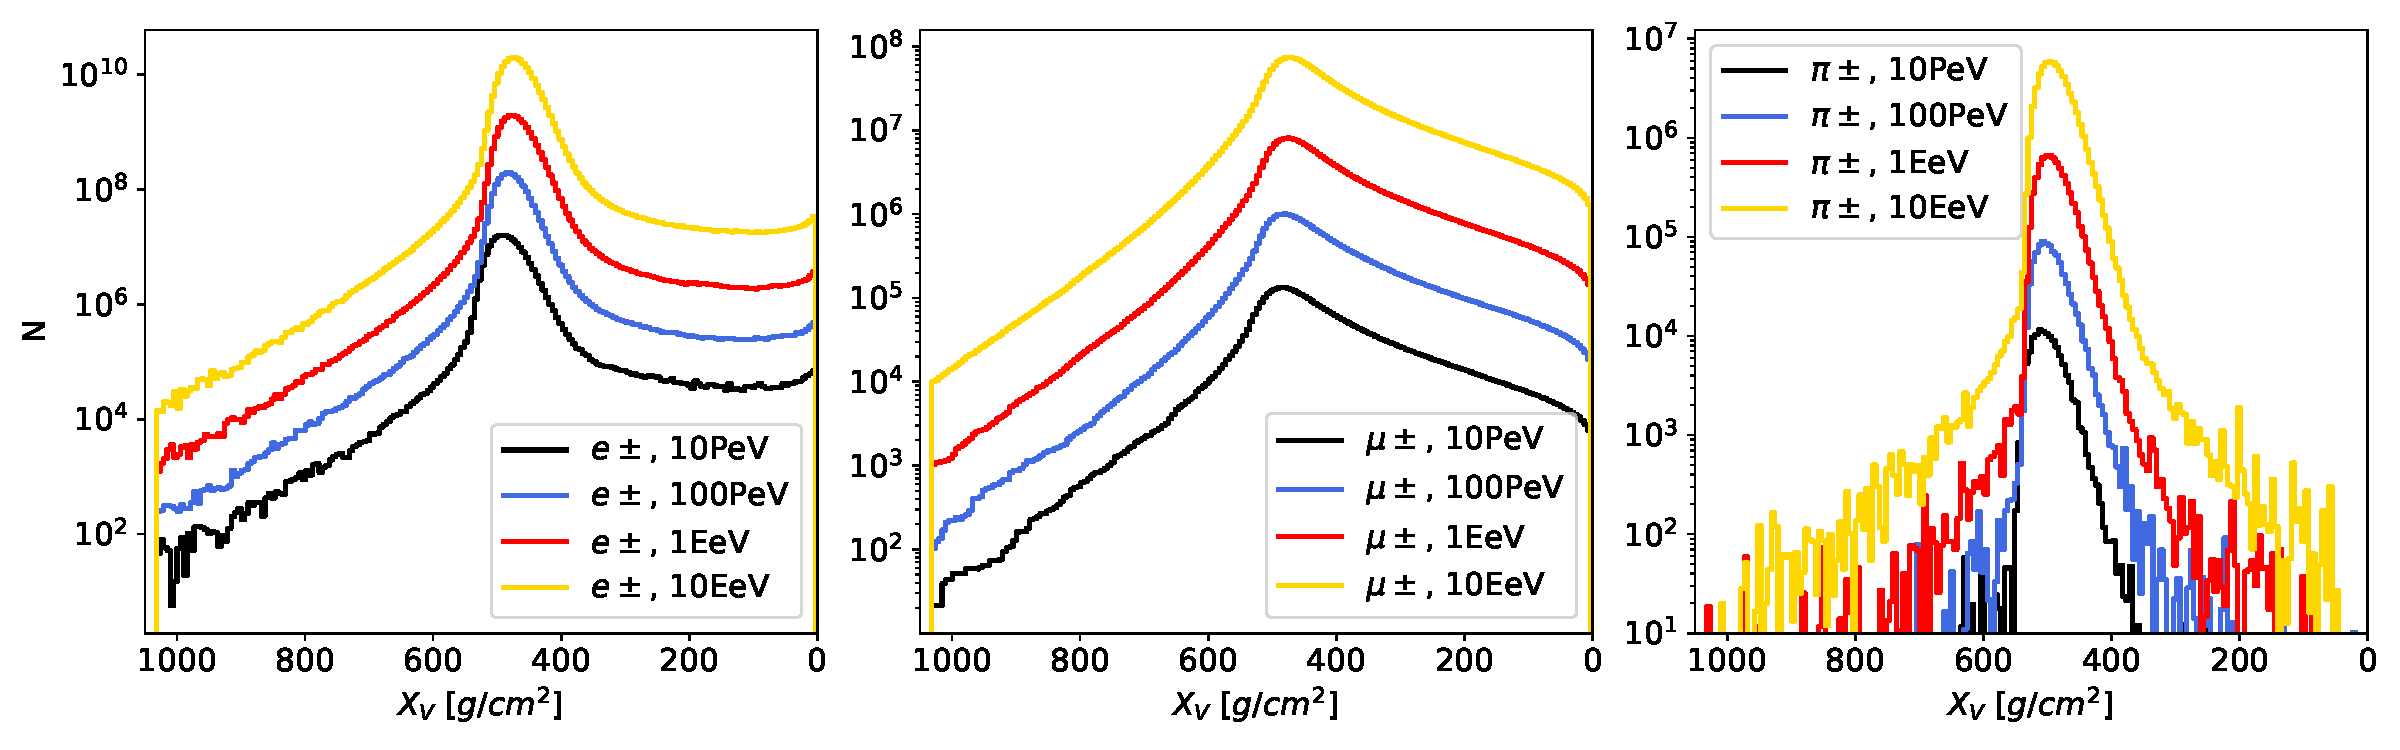
\includegraphics[width=1\linewidth]{figures/cascadas/upgoing_p_varE_95deg_5km_v3}
	\end{figure}
\begin{itemize}
	\item Nº máximo de partículas prácticamente lineal con la energía. En base a modelos \cite{matthews2005heitler}:
	\begin{equation*}
			N_{max}^{e}\propto E_0\;\;;\;\;N_{max}^{\mu}\propto E_0^\beta\;\text{con}\;\beta\sim0,85-0,9
	\end{equation*}
\end{itemize}
\end{frame}

\begin{frame}{Naturaleza del primario (hadrón - leptón)}
	\begin{itemize}
		\item Primario de $1\,\mathrm{EeV}$ a $\theta = 95^\circ$ interaccionando a nivel del suelo.
		\end{itemize}
			\begin{figure}[H]
			\centering
			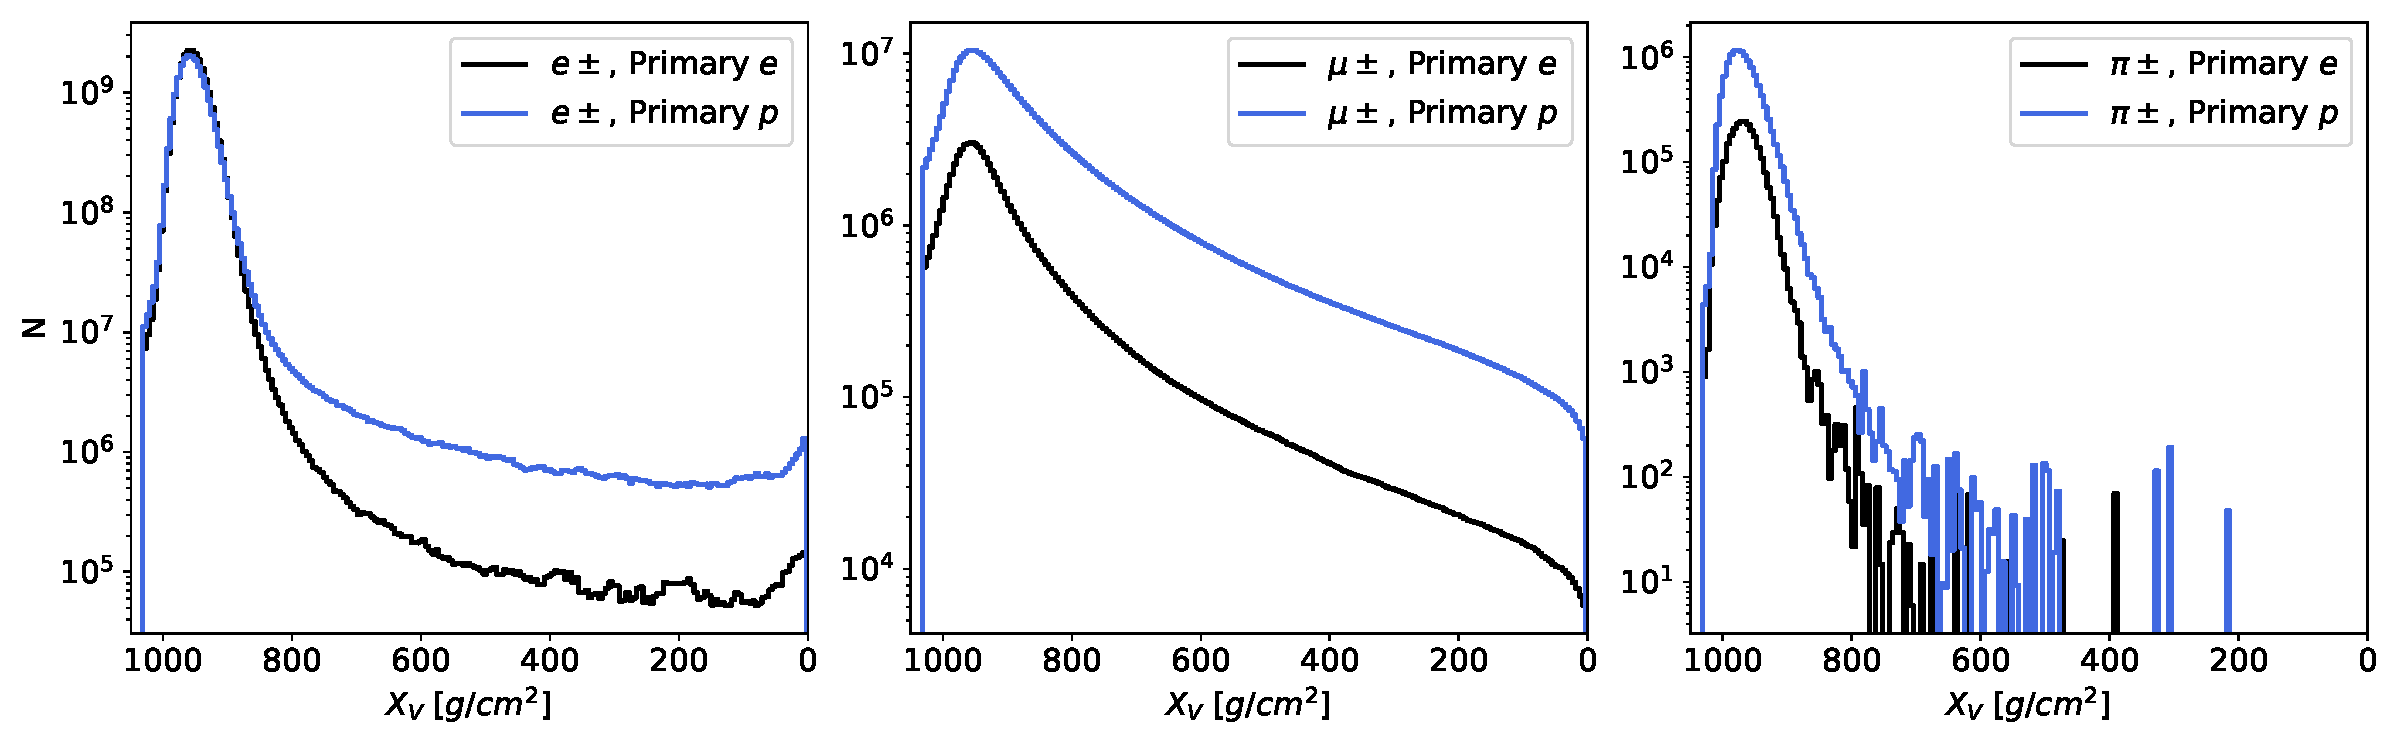
\includegraphics[width=1.\linewidth]{figures/cascadas/upgoing_pe_1EeV_95deg_0km_v2}
		\end{figure}
	\begin{itemize}
		\item Nº máximo de $e^\pm$ muy similar. Nº máximo de $\mu^\pm,\pi^\pm$ menor para primario $e^-$ en un factor $\sim 4$
		\item Cola de $e^\pm$ para primario $p$ $\rightarrow$ Origen en desintegración de $\mu^\pm$
	\end{itemize}
\end{frame}
\begin{frame}{Comparación de cascadas hacia arriba - abajo}
	\begin{itemize}
		\item Protón de $1\,\mathrm{EeV}$ a $\theta=95^\circ \,(85^\circ)$ interaccionando en $h=0\,(100)\,\mathrm{km}$ 
	\end{itemize}
\begin{figure}[H]
	\centering
	\includegraphics[width=.95\linewidth]{figures/comp_ugdg_slides}
\end{figure}
	\begin{itemize}
		\item Producción de más partículas en cascadas hacia arriba (dominio de interacciones).
		\item Menor energía promedio por partícula en cascadas hacia arriba. Las desintegraciones contribuirán antes.
		\item En cascadas hacia arriba, máximo localizado en las proximidades del suelo. (Gran cantidad de materia atravesada en poco tiempo)
	\end{itemize}
\end{frame}
\begin{frame}{Resultados clave}
	\begin{enumerate}
		\item Cascadas atmosféricas hacia arriba $\rightarrow$ elevado número de partículas cargadas en el máximo ($\sim 10^8-10^{10}$), que aumenta con la inclinación de la cascada. 
	\item Número máximo de partículas producidas lineal con la energía del primario. 
	\item La naturaleza del primario no provoca gran diferencia en el número máximo de partículas EM.
	\item Las cascadas hacia arriba presentan máximos muy localizados en las proximidades del nivel del suelo y con una elevada producción de partículas comparadas con cascadas hacia abajo.
	\end{enumerate}
\end{frame}
	\section{Emisión en radio: Principio físico y caracterización}
	\begin{frame}{Origen de la emisión en radio}
	\begin{itemize}
		\item Cascada atmosférica$\rightarrow$ Cargas en movimiento ($v\sim c$) en un medio.
	\end{itemize}
	\begin{block}{}
		\centering\textit{Dos mecanismos de emisión (aparición de corrientes netas)}
	\end{block}
	\begin{columns}
		\column{.45\textwidth}
		\begin{block}{\centering\textit{Deflexión geomagnética}}
			\centering
			$\vect{J}\sim \hat{\vect{n}}_{\text{cascada}}\times\vect{B}$
		\end{block}
		\column{.45\textwidth}
		\begin{block}{\centering\textit{Efecto Askaryan}}
			\centering
			$\vect{J}\sim-\hat{\vect{n}}_{\text{cascada}}$
		\end{block}
	\end{columns}
	\vspace{10mm}
	\begin{itemize}
		\item Puede comprobarse que:
		\begin{itemize} \item $\vect{E}_{rad}\parallel\hat{\vect{R}}\times\left(\hat{\vect{R}}\times\vect{J}\right)$ donde $\vect{R}\equiv$ Posición fuente-observador
			\item Emisión máxima en el ángulo \v{C}erenkov
		\end{itemize}
	\end{itemize}
\end{frame}

\begin{frame}{Origen de la emisión en radio II}

\begin{block}{\centering\textit{Deflexión geomagnética}}
	\centering Campo magnético terrestre $\vect{B}$ (deflexión de cargas según signo)
	$$\vect{J}\sim \hat{\vect{n}}_{\text{cascada}}\times\vect{B}j$$  
\end{block}

\begin{columns}
	\column{.5\textwidth}
	
	\begin{figure}[H]
		\centering
		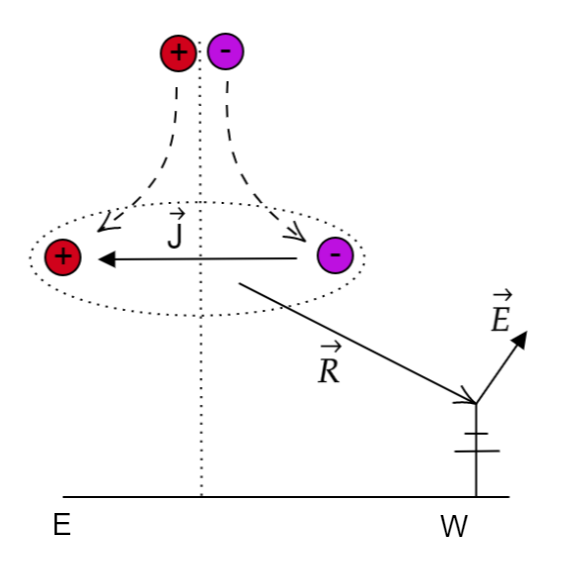
\includegraphics[width=.6\linewidth]{figures/Geomag_deflexion_1}
	\end{figure}
	\column{.5\textwidth}
	\begin{figure}[H]
		\centering
		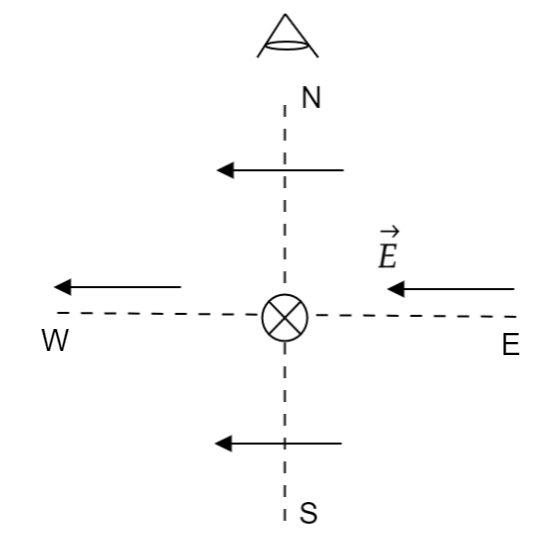
\includegraphics[width=.6\linewidth]{figures/Geomag_deflexion_2}
	\end{figure}
\end{columns}
\end{frame}
\setcounter{page}{14}
\begin{frame}{Origen de la emisión en radio III}
	
	\begin{block}{\centering\textit{Efecto Askaryan}}
			\centering Aparición de carga neta a lo largo del eje (e.g. aniquilación $e^+e^-$)
			$$\vect{J}\sim-\hat{\vect{n}}_{\text{cascada}}$$
		\end{block}
	
	\begin{columns}
		\column{.5\textwidth}
		
		\begin{figure}[H]
			\centering
			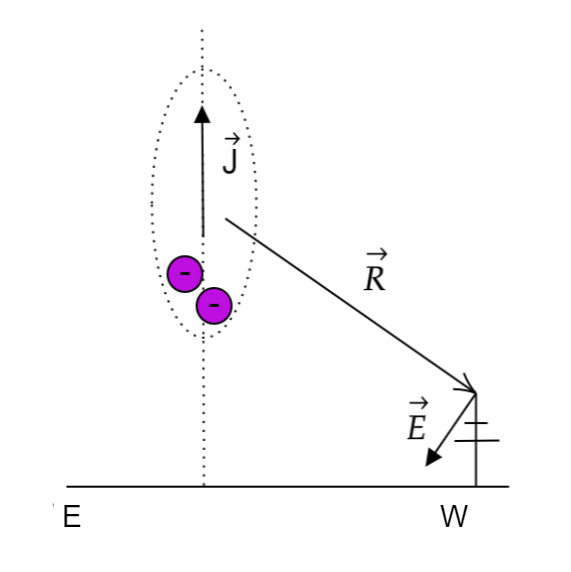
\includegraphics[width=.6\linewidth]{figures/Askaryan_1}
		\end{figure}
		\column{.5\textwidth}
		\begin{figure}[H]
			\centering
			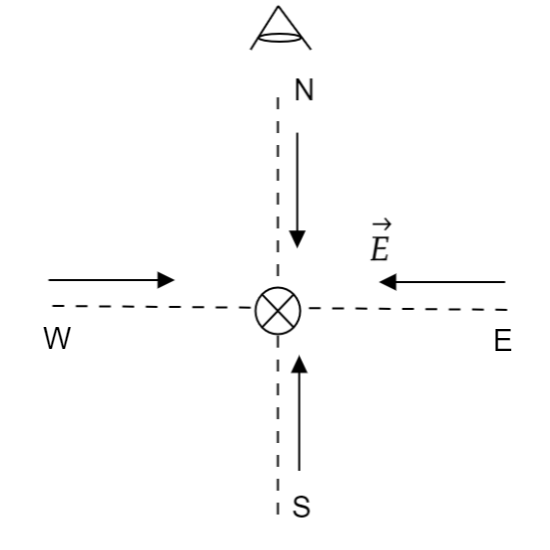
\includegraphics[width=.6\linewidth]{figures/Askaryan_2}
		\end{figure}
	\end{columns}
\end{frame}

	\begin{frame}{Caracterización en simulaciones con ZHAireS}
		\begin{itemize}
			\item Simulación de la emisión en radio: ZHAireS (AIRES $+$ algoritmo ZHS) $\rightarrow$ Primeros principios del EM, cálculo numérico a nivel microscópico.
			\item Componente EW de campo al N del core de una cascada vertical (Primario $p$ de $10^{17}\,\mathrm{eV}$):
		\end{itemize}
	\begin{columns}
		\column{.45\textwidth}
		\begin{figure}[H]
			\centering
			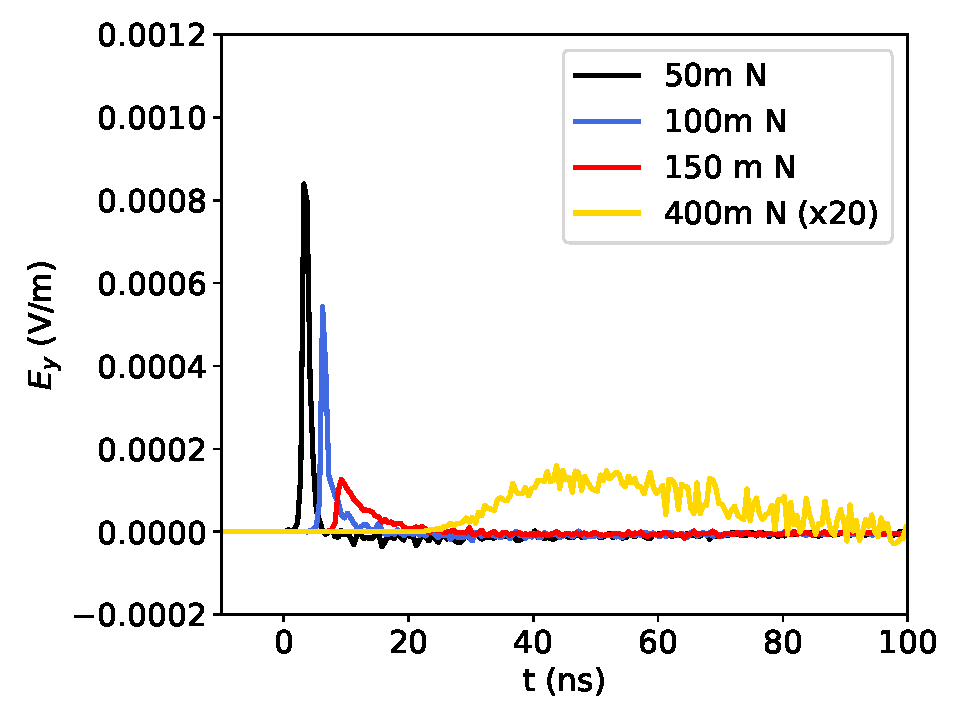
\includegraphics[width=.95\linewidth]{figures/radio/p_1e17_0deg_EW_N_v2}
		\end{figure}
	\begin{block}{}
		\centering\textit{Pulso bipolar, $\sim 10 \,\mathrm{ns}$}
	\end{block}
\column{.45\textwidth}
\begin{figure}[H]
	\centering
	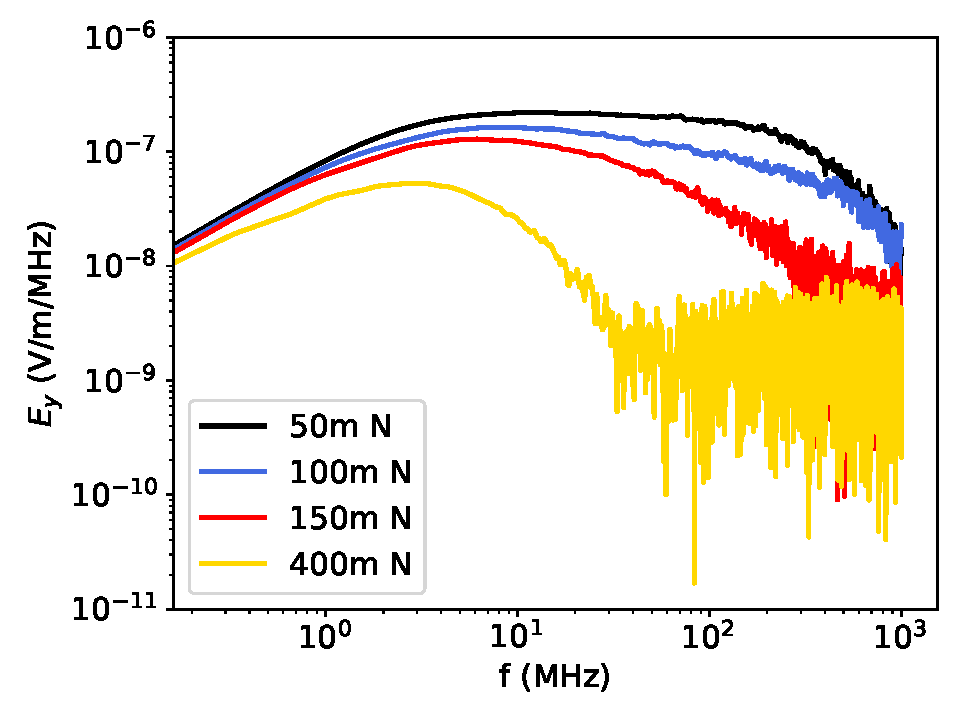
\includegraphics[width=.95\linewidth]{figures/radio/p_1e17_0deg_EW_N_Fourier_v3}
\end{figure}
\begin{block}{}
	\centering\textit{Emisión coherente hasta $\sim10-100\,\mathrm{MHz}$ (RF)}
\end{block}
	\end{columns}
	\end{frame}
\begin{frame}{Caracterización en simulaciones con ZHAireS II}
	\begin{itemize}
		\item Ejemplo de cascada inclinada: Primario $p$ de $10^{19}\,\mathrm{eV}$ a $\theta = 70^\circ$
		\item Señal máxima observando el máximo del desarrollo bajo el ángulo \v{C}erenkov 
	\end{itemize}
	\begin{figure}[H]
		\centering
		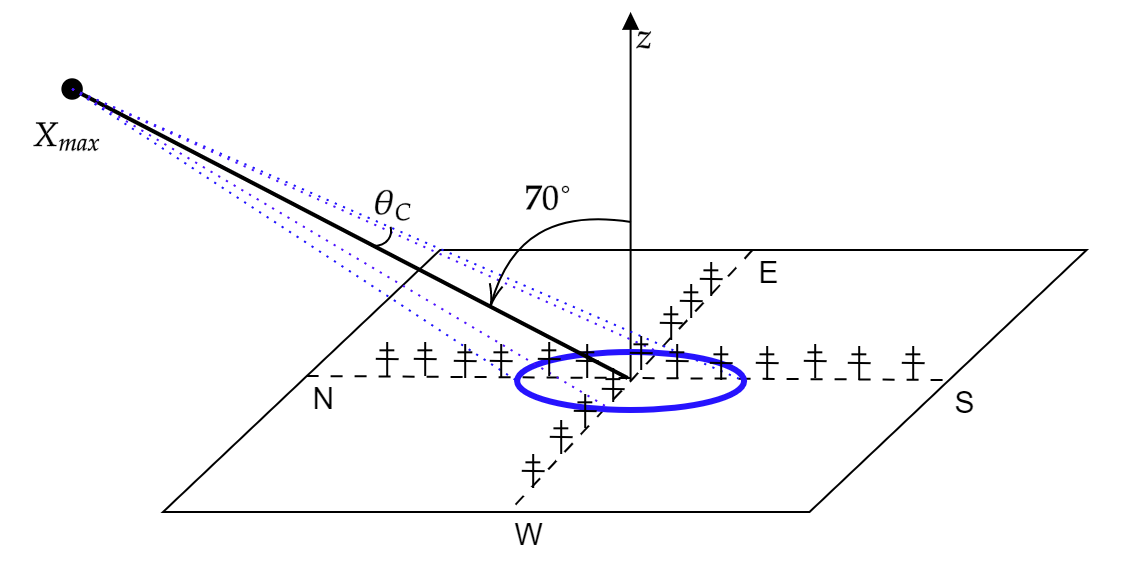
\includegraphics[width=.7\linewidth]{figures/radio/ANITApaper_showscheme}
	\end{figure}
\end{frame}

\begin{frame}{Caracterización en simulaciones con ZHAireS III}
	\begin{columns}
		\column{.49\textwidth}
	\begin{figure}[H]
		\centering
		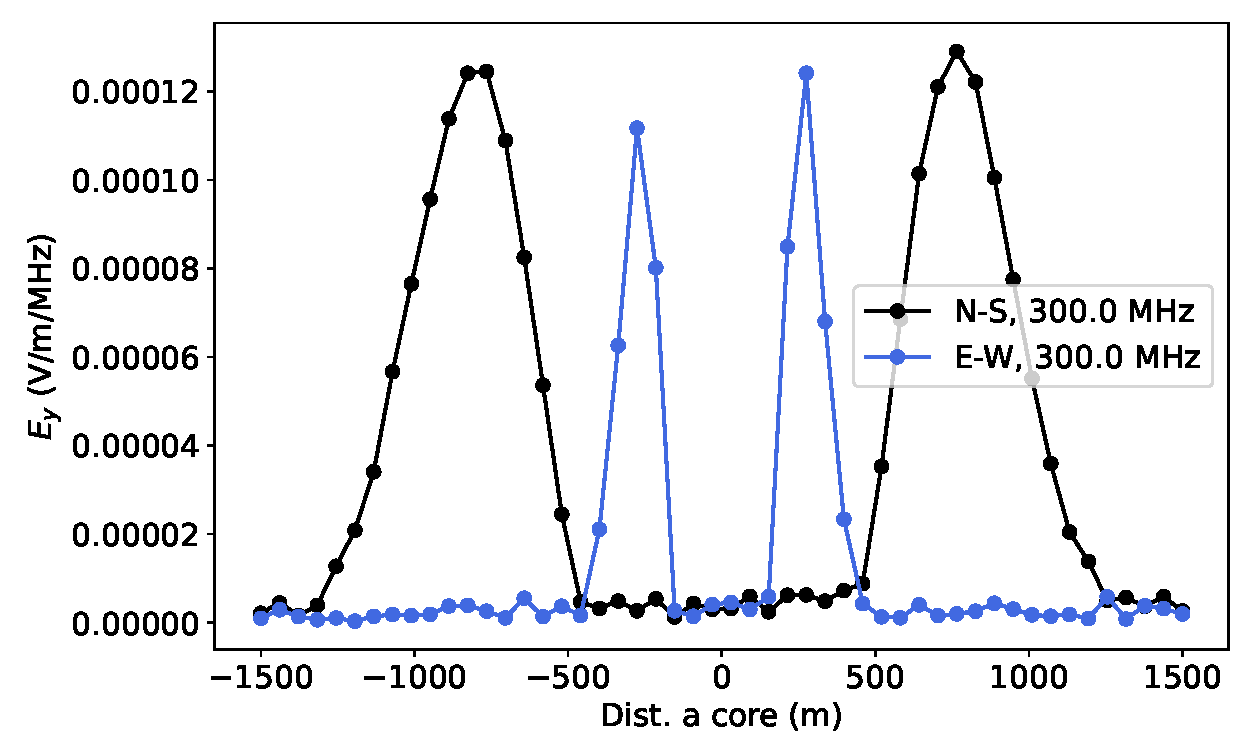
\includegraphics[width=.95\linewidth]{figures/radio/downgoing_p_10EeV_70deg_Ey_300MHz_ground_v2}
	\end{figure}
		\column{.49\textwidth}
\begin{figure}[H]
	\centering
	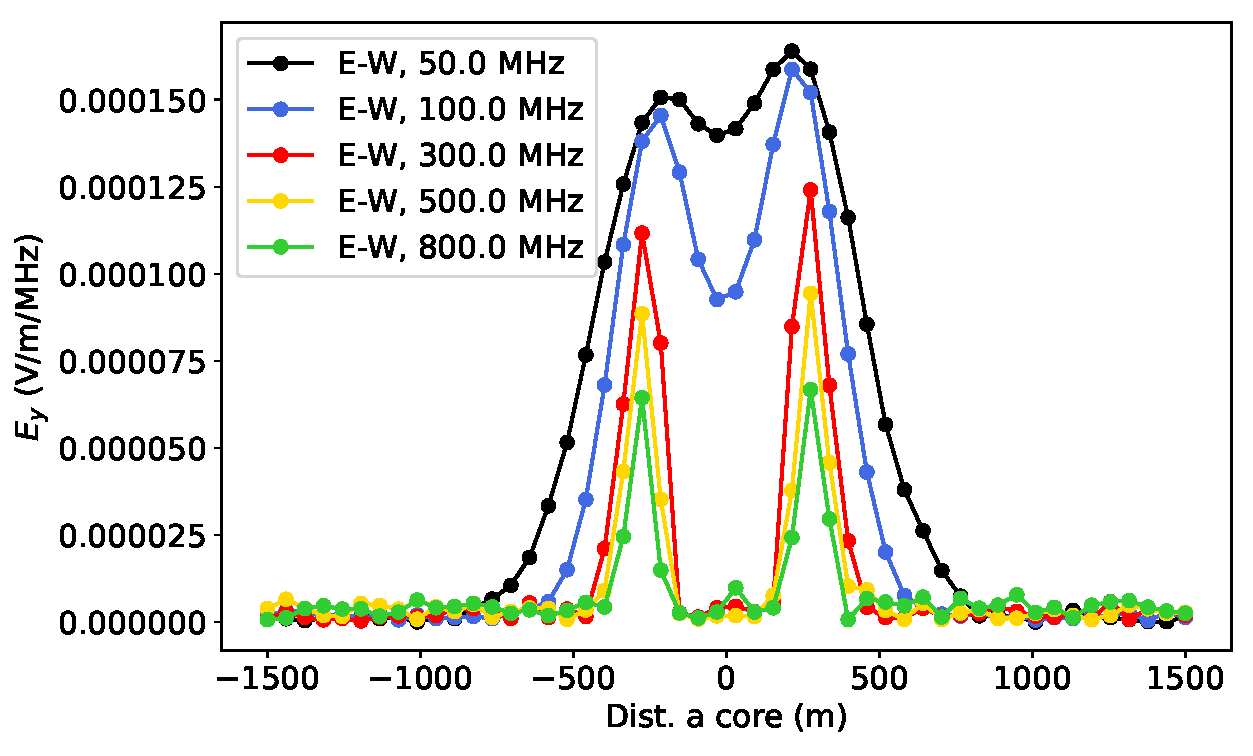
\includegraphics[width=.95\linewidth]{figures/radio/downgoing_p_10EeV_70deg_Ey_varfreq_groundEW_v2}
\end{figure}
	\end{columns}
\pause\begin{block}{\centering\textit{Ideas clave}}
	\begin{itemize}
		\item Contribuciones geomagnética + Askaryan (diferente polarización)
		\item Frecuencias de interés (coherencia): Banda $\sim 10-100\,\mathrm{MHz}$
		\item Emisión máxima en \textit{elipse} \v{C}erenkov. Definición mayor a mayor frecuencia.
	\end{itemize}
\end{block}
\end{frame}
	\section{Emisión en radio en cascadas hacia arriba}


\begin{frame}{Casos simulados}
	\begin{itemize}
		\item $\text{Desintegraciones del leptón } \tau\rightarrow\left\{\begin{array}{l}\text{Hadrones}+\nu_\tau\; (\sim64\%)\\e\nu_e\nu_\tau\;(\sim 17\%)\\\mu \nu_\mu\nu_\tau\;(\sim 17\%)\end{array}\right.$
		\item Poca influencia de la naturaleza del primario en el máximo $\rightarrow$ Primario $p$ interaccionando a $0\,\mathrm{km}$ de altura.
		\item Evento realista $\rightarrow$ Cascada hacia arriba muy inclinada, $\theta = 95^\circ$
		\pause\begin{columns}
					\column{.32\textwidth}
			\begin{block}{\centering Altura de obs.}
				\centering $5\,\mathrm{km}$ (BEACON)\\$36\,\mathrm{km}$ (PUEO)\\$100\,\mathrm{km}$
			\end{block}
			\column{.32\textwidth}
			\begin{block}{\centering Energía del primario}
				\centering $10\,\mathrm{PeV}$\\$100\,\mathrm{PeV}$\\$1\,\mathrm{EeV}$
			\end{block}

	\column{.32\textwidth}
	\begin{block}{\centering Frecuencia}
		\centering $100\,\mathrm{MHz}$\\$300\,\mathrm{MHz}$\\$500\,\mathrm{MHz}$
	\end{block}
		\end{columns}
	\end{itemize}
\end{frame}

\begin{frame}{Resultados: Altura de observación}
	\begin{figure}[H]
		\centering
		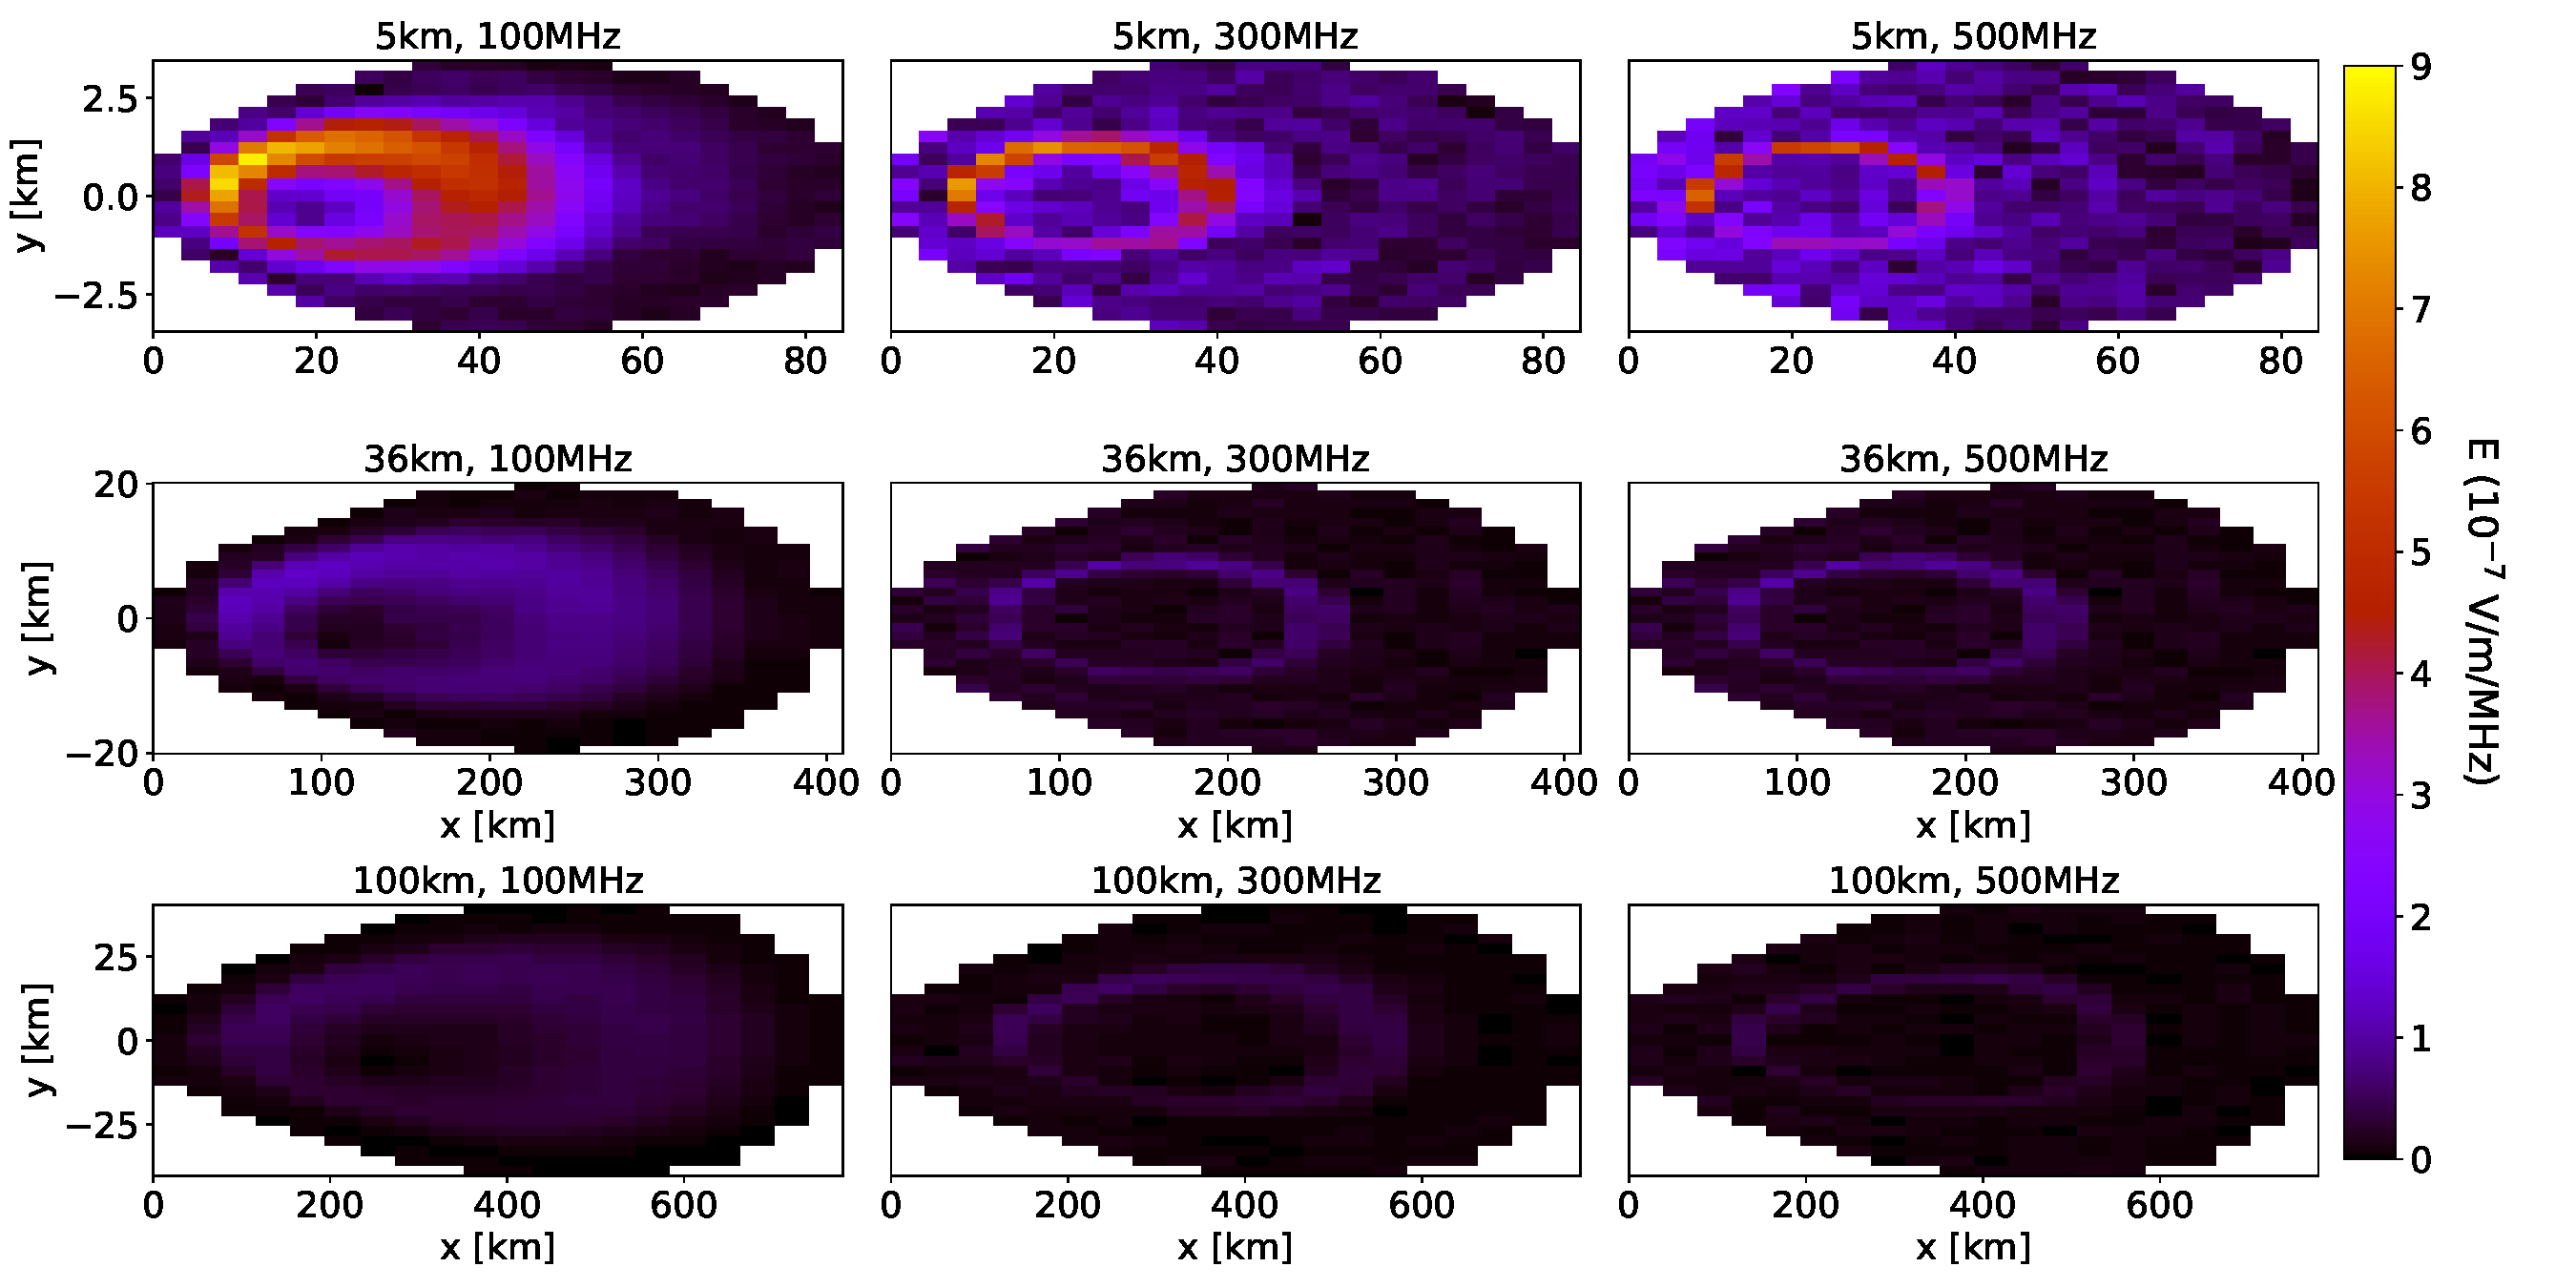
\includegraphics[width=1\linewidth]{figures/Radio_UG/85deg_varh_5_36_100}
	\end{figure}
\end{frame}

\begin{frame}{Resultados: Energía del primario}
		\begin{figure}[H]
		\centering
		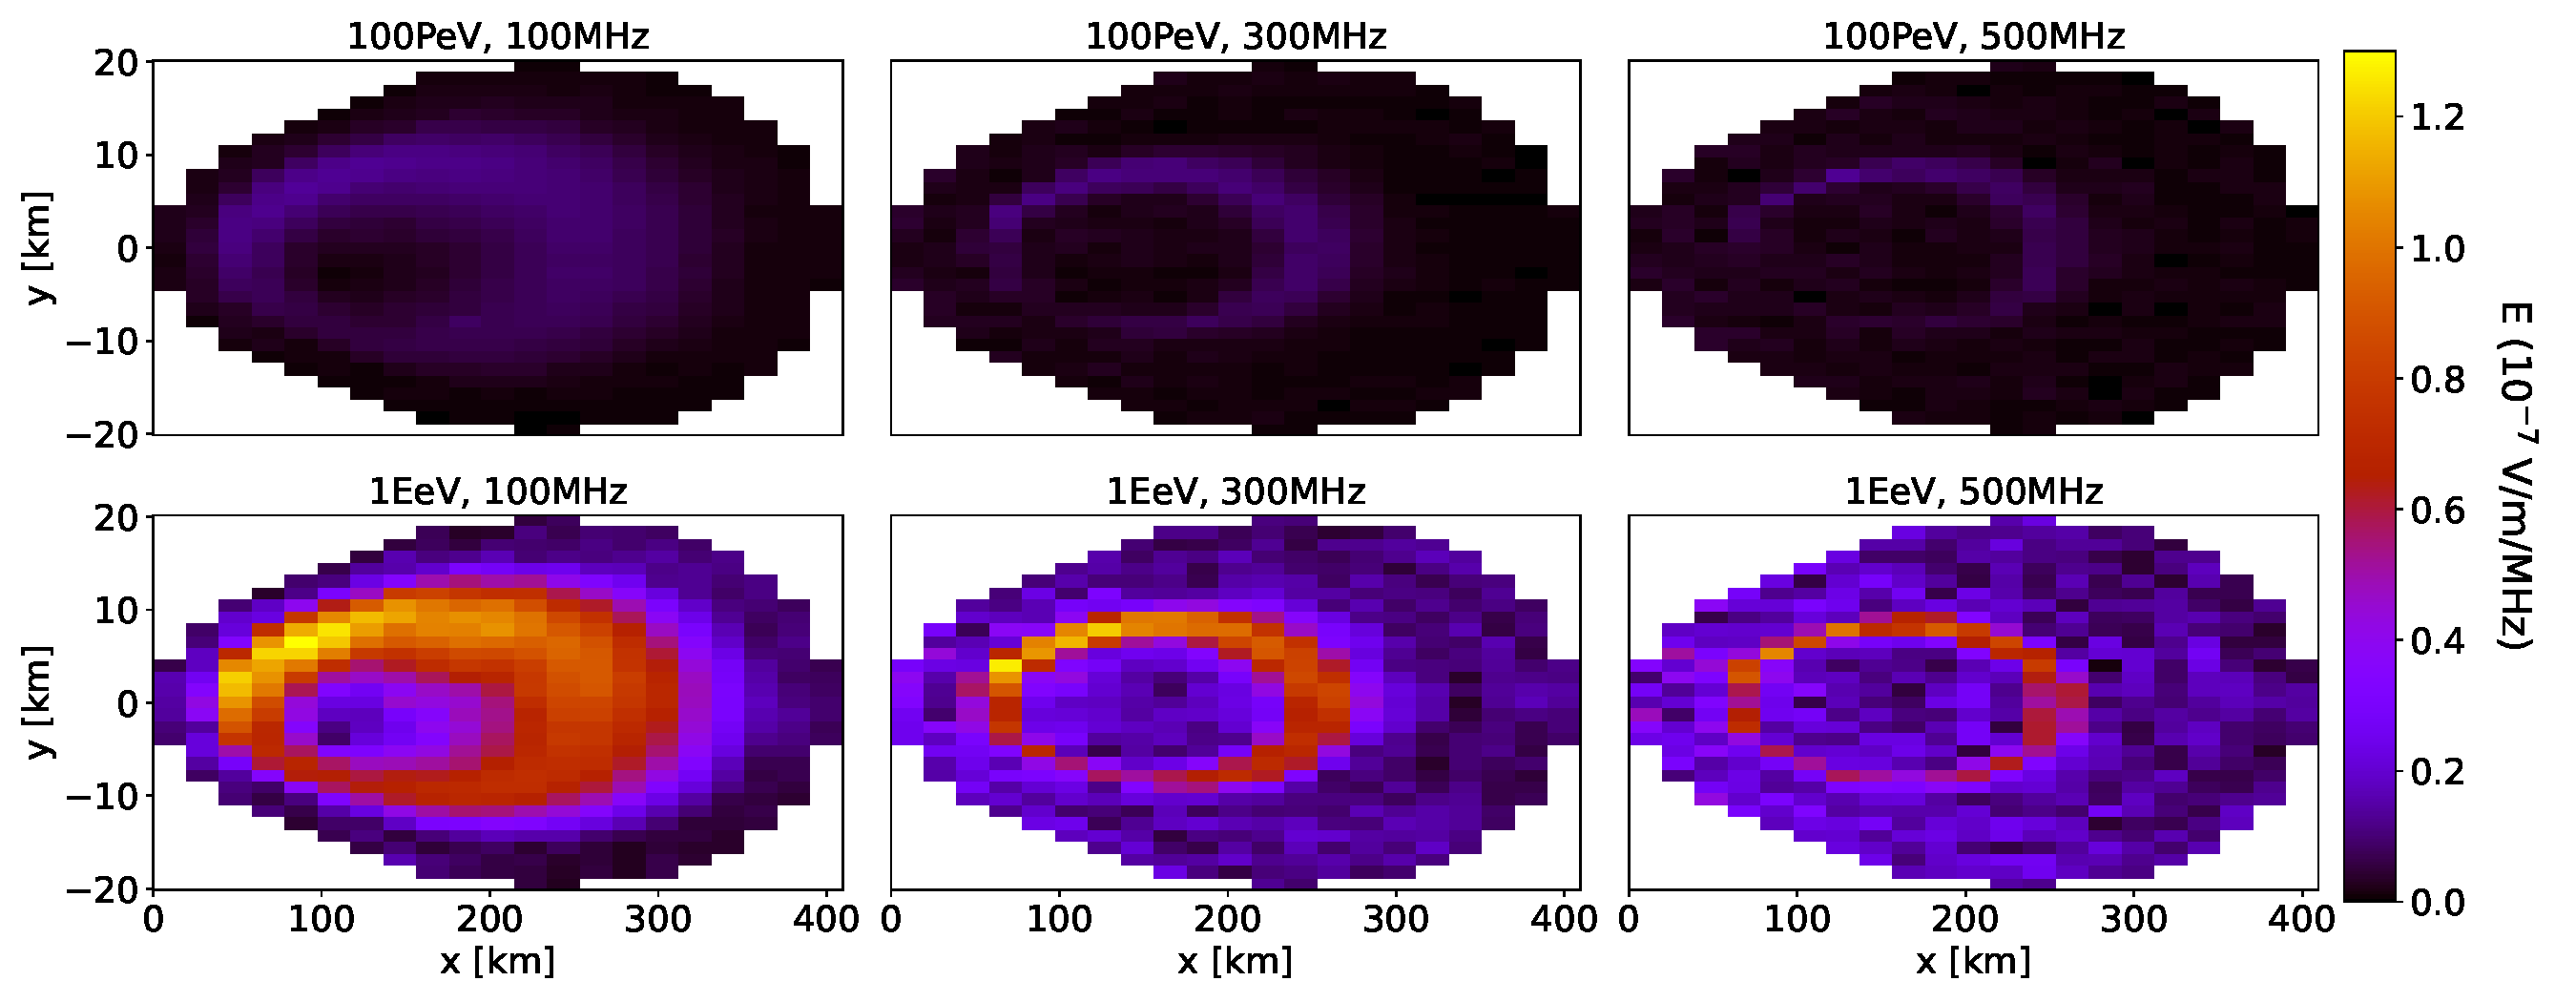
\includegraphics[width=1\linewidth]{figures/Radio_UG/85deg_varE}

	\end{figure}
\end{frame}
	\begin{frame}{Emisión en radio en cascadas hacia arriba}
	\begin{itemize}
		\item Desarrollo hacia arriba en la atmósfera y observación de la radiación por encima del máximo $\rightarrow$ Asimetría opuesta a cascadas hacia abajo
	\end{itemize}
	\begin{figure}[H]
		\centering
		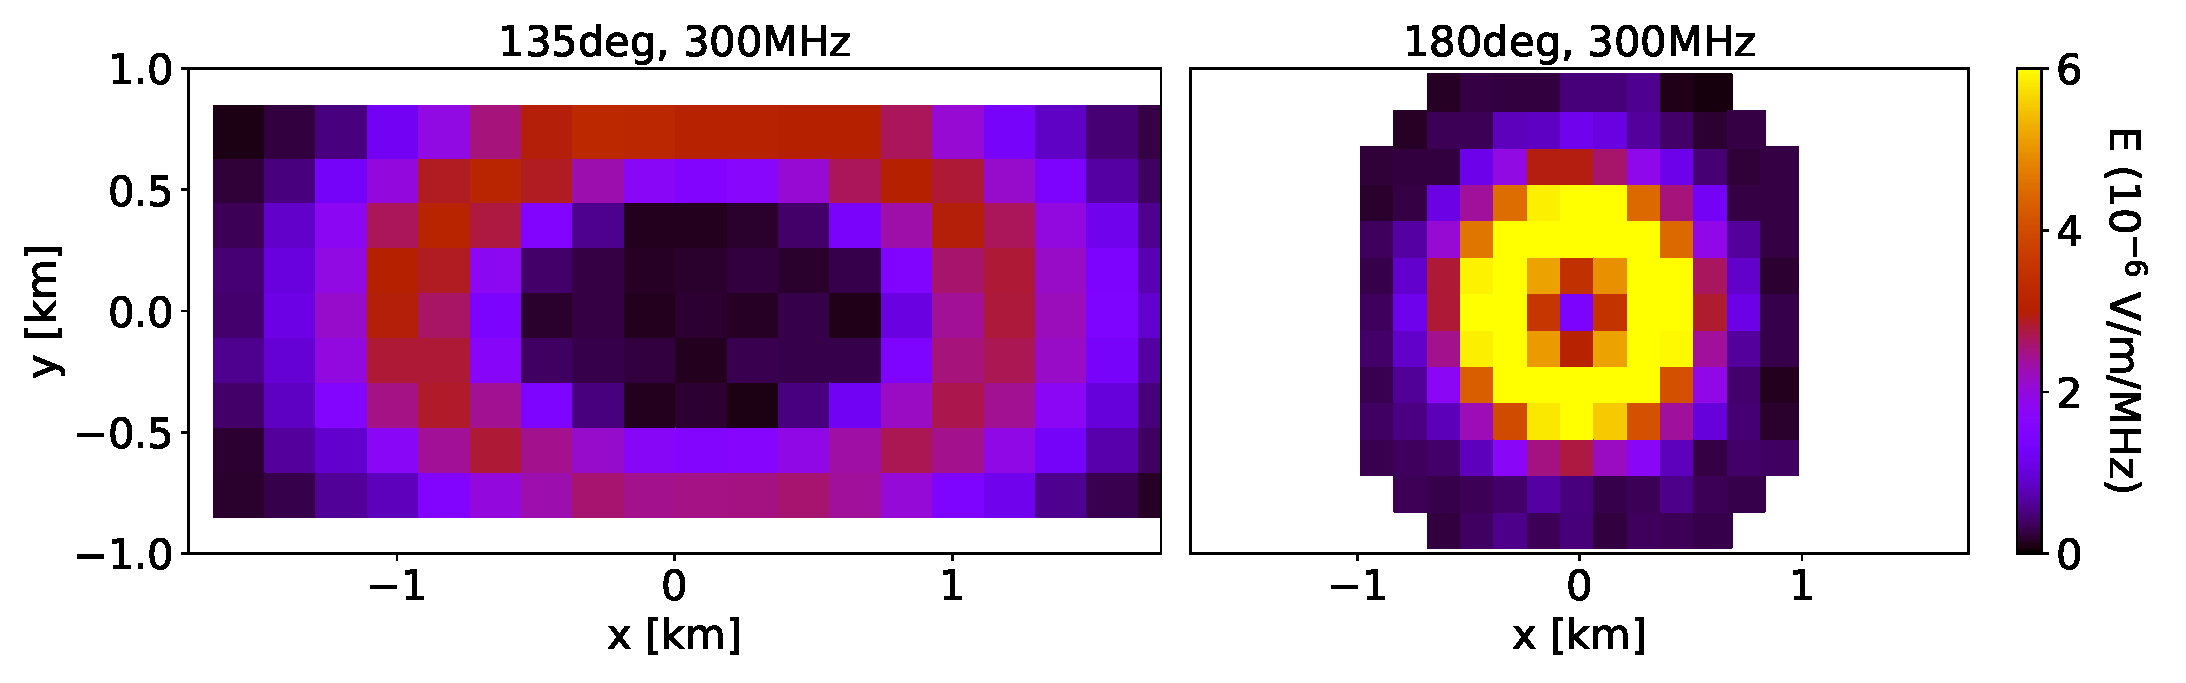
\includegraphics[width=.75\linewidth]{figures/Radio_UG/Comparativa_0_45deg}
	\end{figure}
	\begin{figure}[H]
		\centering
		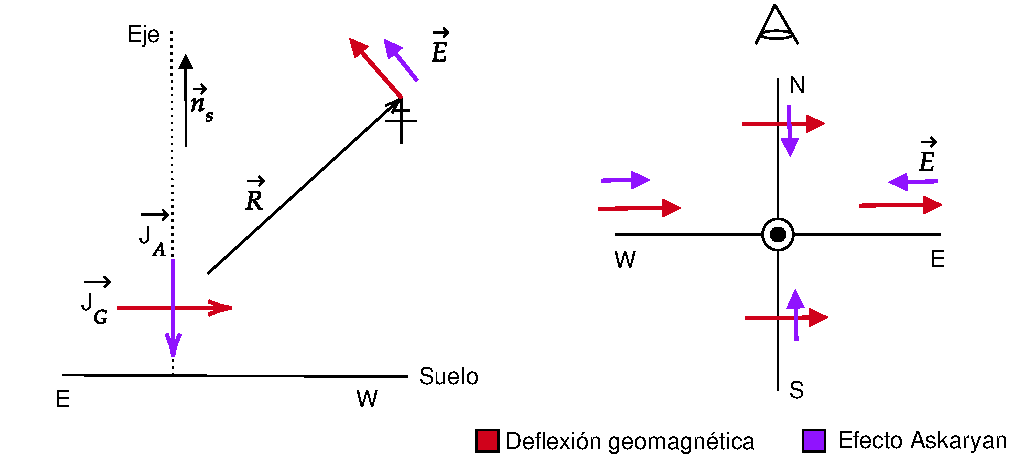
\includegraphics[width=.65\linewidth]{figures/Radio_UG/Polarizacion_UG}
	\end{figure}
	
\end{frame}
\begin{frame}{Propiedades del primario a partir de la señal}
	\begin{itemize}
		\item Elipse \v{C}erenkov $\leftrightarrow$ Naturaleza del primario y dirección de llegada.
		\item Observación de la elipse en arrays de detectores, estudio de retardos en señal $\rightarrow$ \textbf{Dirección de llegada} (técnicas interferométricas)
		\item Dimensiones del patrón $\rightarrow$ Posición del máximo (vértice) $\rightarrow$ \textbf{Naturaleza del primario} (masa)
		\item Dirección de llegada \textit{debajo del horizonte} $\Longleftrightarrow$ Neutrino tau
	\end{itemize}
\end{frame}

\begin{frame}{Propiedades del primario a partir de la señal II}
	\begin{itemize}
		\item Magnitud del campo $\leftrightarrow$ Energía, naturaleza y dirección de llegada del primario 
	\end{itemize}
\begin{columns}
	\column{.47\textwidth}
	\begin{figure}[H]
		\centering
		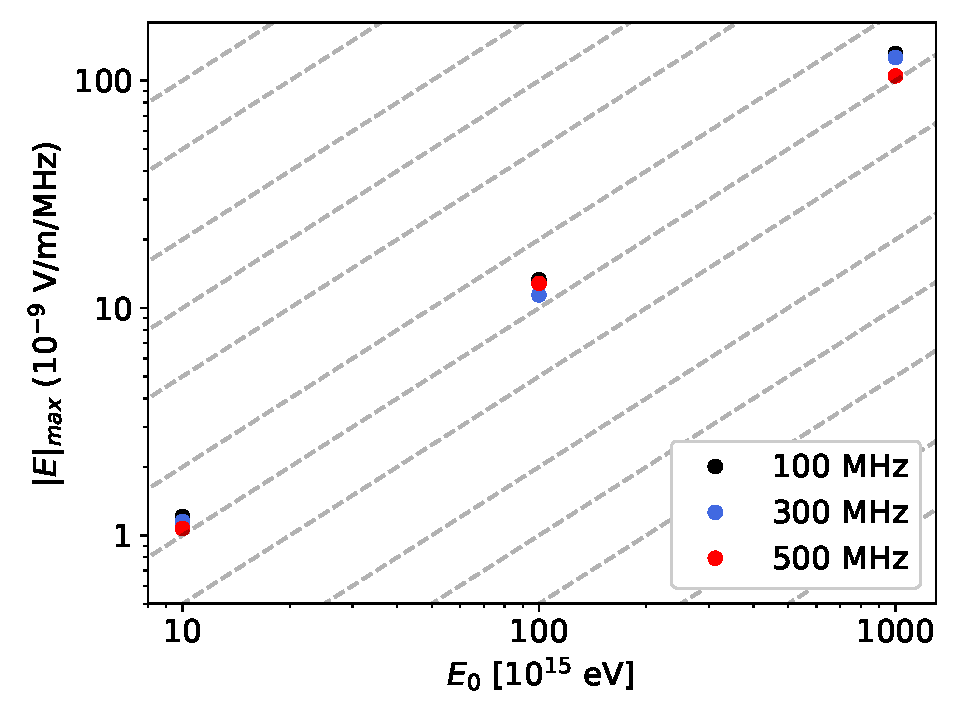
\includegraphics[width=1\linewidth]{figures/Radio_UG/85deg_varE_36km_Emax_vs_E}
	\end{figure}
\begin{block}{}
	\centering $\left|\vect{E}\right|_{max}\propto N_{e}^{max}\propto E_0$\\Dependencia lineal con la energía del primario
\end{block}
	\column{.47\textwidth}
	\begin{figure}[H]
		\centering
		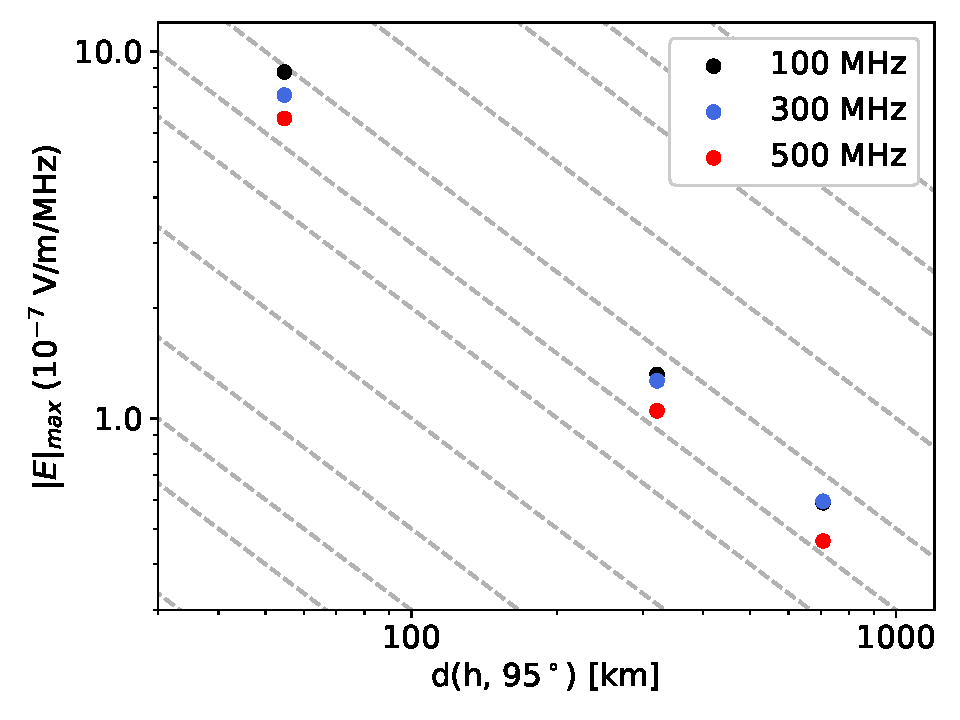
\includegraphics[width=1\linewidth]{figures/Radio_UG/85deg_1EeV_varh_Emax_vs_d}
	\end{figure}
\begin{block}{}
	\centering Dependencia $1/d$ con la distancia al máximo (radiación). Información sobre naturaleza y dirección.
\end{block}
\end{columns}
\end{frame}
	\section{Conclusiones}
	\begin{frame}{Conclusiones}
\begin{enumerate}
	\item Observación de neutrinos de muy altas energías y origen astrofísico como objetivo científico clave. 
	\item Radiodetección $\rightarrow$ Monitorización de grandes áreas, Tierra como blanco de interacción.
	\item Posibilidad de extraer información acerca del primario a partir de la radiación electromagnética emitida en cascadas atmosféricas.
	\item Experimentos planeados, técnicas de análisis avanzadas (interferometría, estudio de flujos de energía y espectro de frecuencias, ...)
\end{enumerate}
	\end{frame}
	
	\begin{frame}[plain, noframenumbering, allowframebreaks]{Referencias}
		\fontsize{9pt}{1}
		\nocite{*}
		\bibliography{TFMbib}
		\bibliographystyle{apalike}
	\end{frame}

\begin{frame}[noframenumbering]{Aux.: Desintegración vs. interacción}
	\begin{itemize}
		\item Distancia de interacción, $\lambda_I\,\left[\mathrm{g/cm^2}\right]$. En uds. de distancia, $d_I\sim\lambda_I/\rho(h)$.
		\item  Distancia de desintegración, $d_{dec}\,\left[\mathrm{m}\right]$: $$d_{dec}=\Gamma\beta c\tau\sim\frac{E}{mc^2}c\tau\left\{\begin{array}{l}\pi^\pm\rightarrow d_{dec}=\Gamma\left(7,8 \,\mathrm{m}\right)\\
			\pi^0\rightarrow d_{dec}=\Gamma\left(2,5\times10^{-8}\,\mathrm{m}\right)\end{array}\right.\;.$$
		\item Energía a la que comienzan a dominar desintegraciones: $$d_{dec}\sim\lambda_I/\rho\implies E_{dec}\sim \frac{\lambda_I mc^2}{\rho c \tau} \;.$$
	\end{itemize}
\end{frame}
\begin{frame}[noframenumbering]{Interacciones en AIRES v. 2.8.4a}
	\begin{table}[H]
		\centering
		\begin{tabular}{lll}
			\hline
			\multicolumn{2}{l}{Partícula}                                                                   & Interacciones                         \\ \hline
			\multicolumn{2}{l}{\multirow{5}{*}{\begin{tabular}[c]{@{}c@{}}$\gamma$\\ $e^\pm$\end{tabular}}} & Efectos Compton y fotoeléctrico       \\
			\multicolumn{2}{l}{}                                                                            & Bremsstrahlung y producción de pares  \\
			\multicolumn{2}{l}{}                                                                            & Aniquilación $e^+e^-$                 \\
			\multicolumn{2}{l}{}                                                                            & Emisión de $e^-$ knock-on (scattering M\o{}ller, Bhabha)            \\
			\multicolumn{2}{l}{}                                                                            & Reacciones fotonucleares, ...         \\ \hline
			\multicolumn{2}{l}{\multirow{3}{*}{$\mu^\pm$}}                                                  & Bremsstrahlung y producción de pares  \\
			\multicolumn{2}{l}{}                                                                            & Emisión de $e^-$ knock-on             \\
			\multicolumn{2}{l}{}                                                                            & Desintegración                        \\ \hline
			\multicolumn{2}{l}{$\nu$'s}                                                                   & Aparición en desintegraciones         \\ \hline
			\multicolumn{2}{l}{$p,\bar p, n, \bar n, \Lambda$}                                              & Colisiones hadrónicas y núcleo-núcleo \\
			\multicolumn{2}{l}{$\pi^0, \pi^\pm, K^0_{L,S}, K^\pm$}                                          & Emisión de $e^-$ knock-on             \\
			\multicolumn{2}{l}{Núcleos $Z\leq 36$}                                                          & Desintegraciones                      \\ \hline
		\end{tabular}
	\end{table}
\end{frame}
\begin{frame}[noframenumbering]{Aux.: Materia atravesada vs. $\theta$}
	$$X_{s}^\text{up}(h,\theta)=\int_{0}^h\rho(h')dl=\int_0^{h}\rho(h')\frac{dh'}{\sqrt{1-\frac{R_T^2\sin^2{\theta}}{\left(R_T+h'\right)^2}}}\;.$$
	\begin{figure}[H]
		\centering
		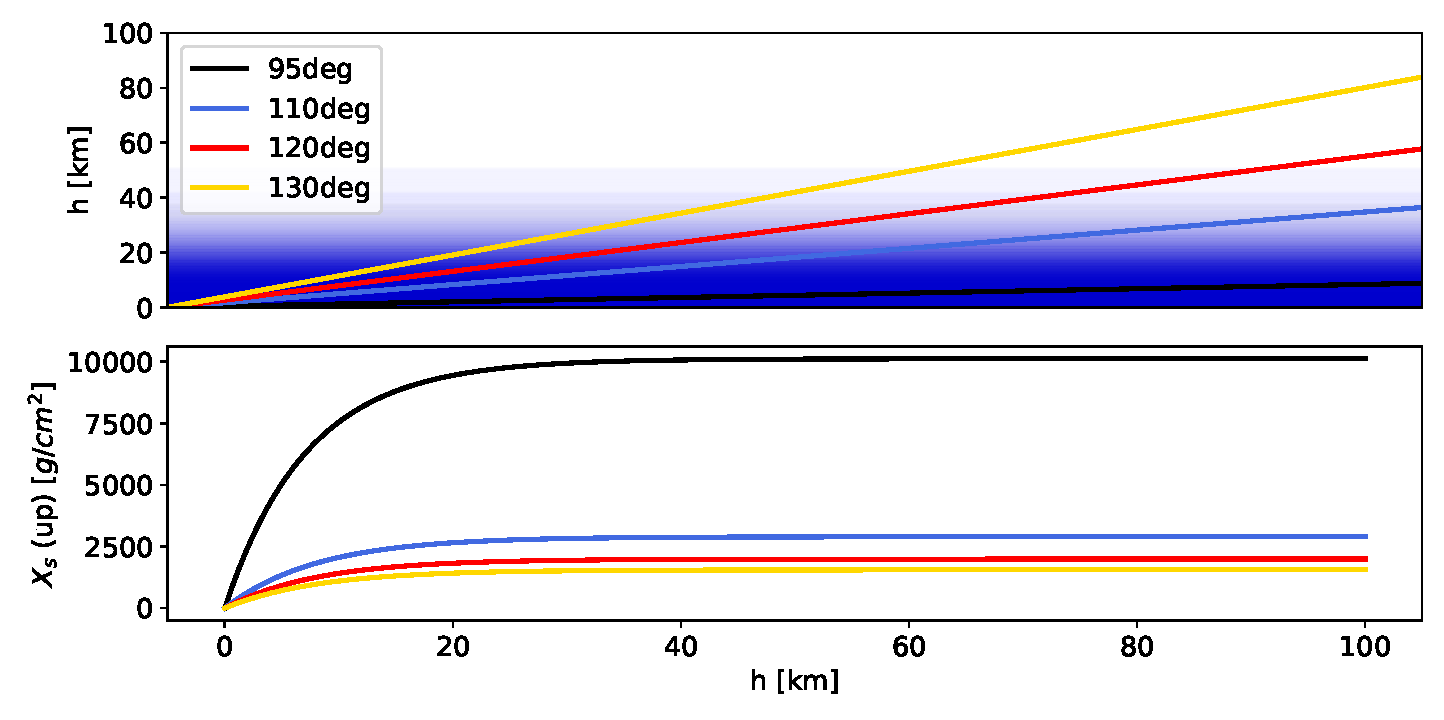
\includegraphics[width=.8\linewidth]{figures/cascadas/ProfAtravesadavsang}
	\end{figure}
\end{frame}
\begin{frame}[noframenumbering]{Aux.: Altura de interacción en cascadas hacia arriba}
		\begin{figure}[H]
	\centering
	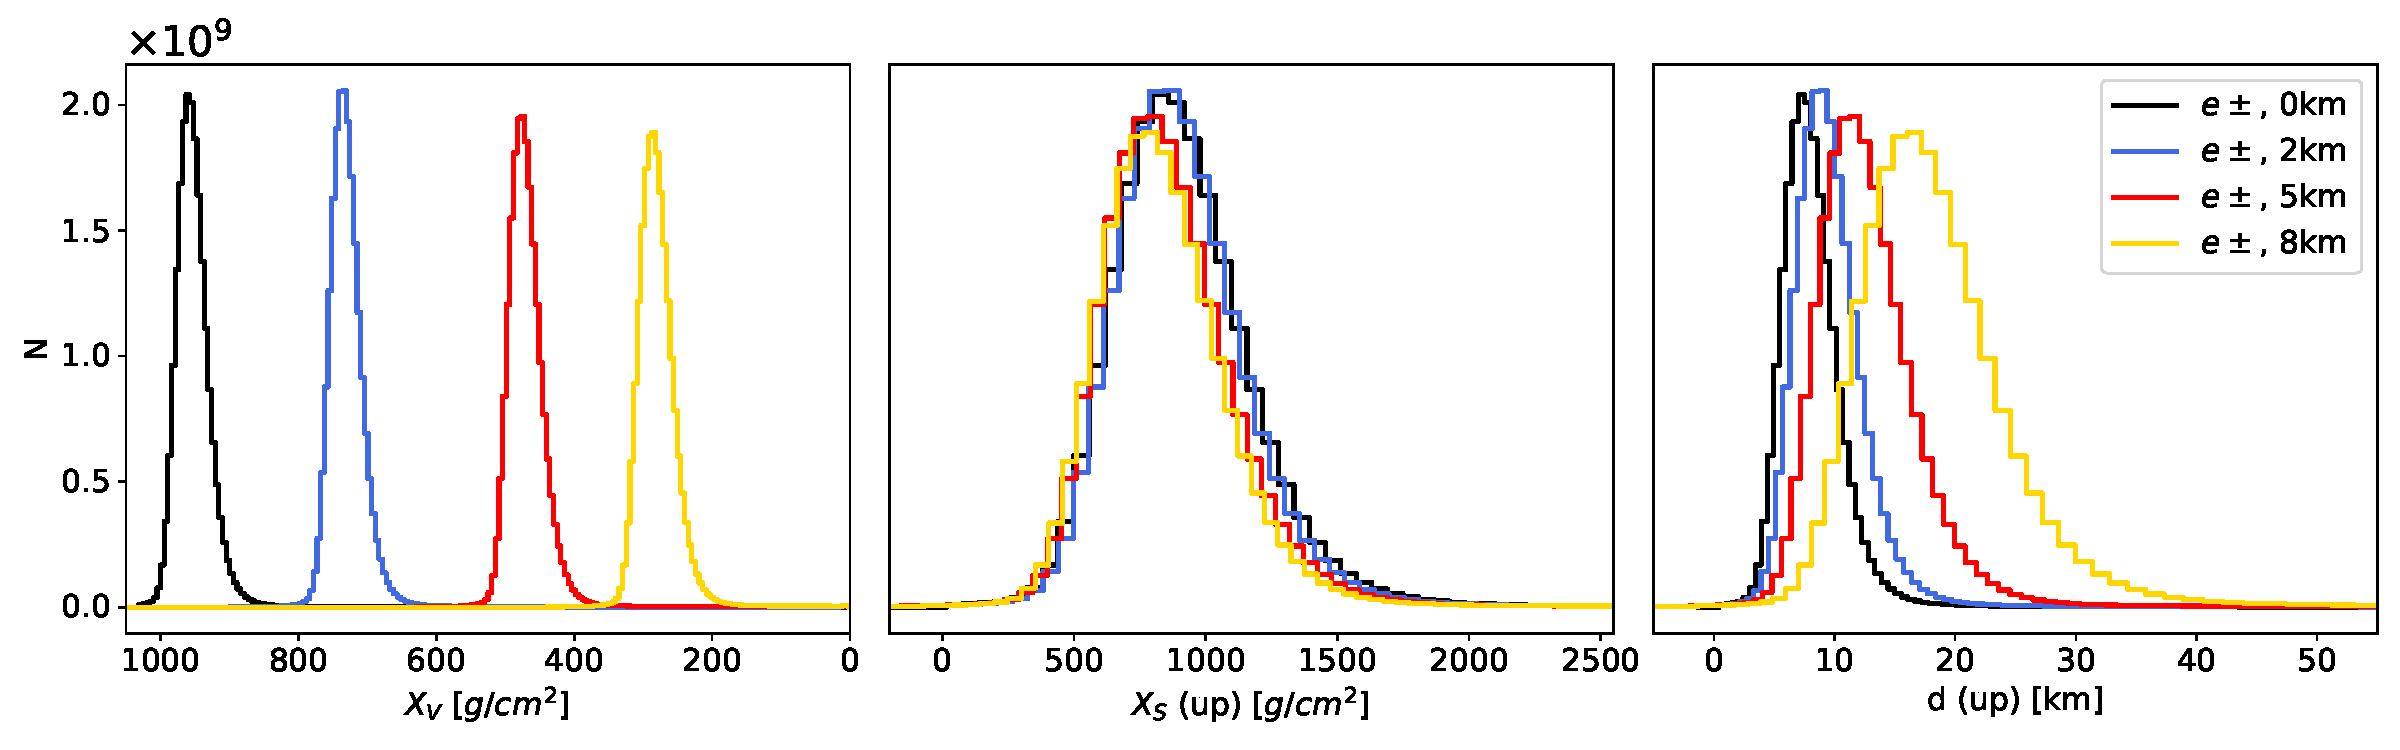
\includegraphics[width=.95\linewidth]{figures/cascadas/upgoing_p_1EeV_95deg_varh_e_v2}
\end{figure}
\begin{figure}[H]
	\centering
	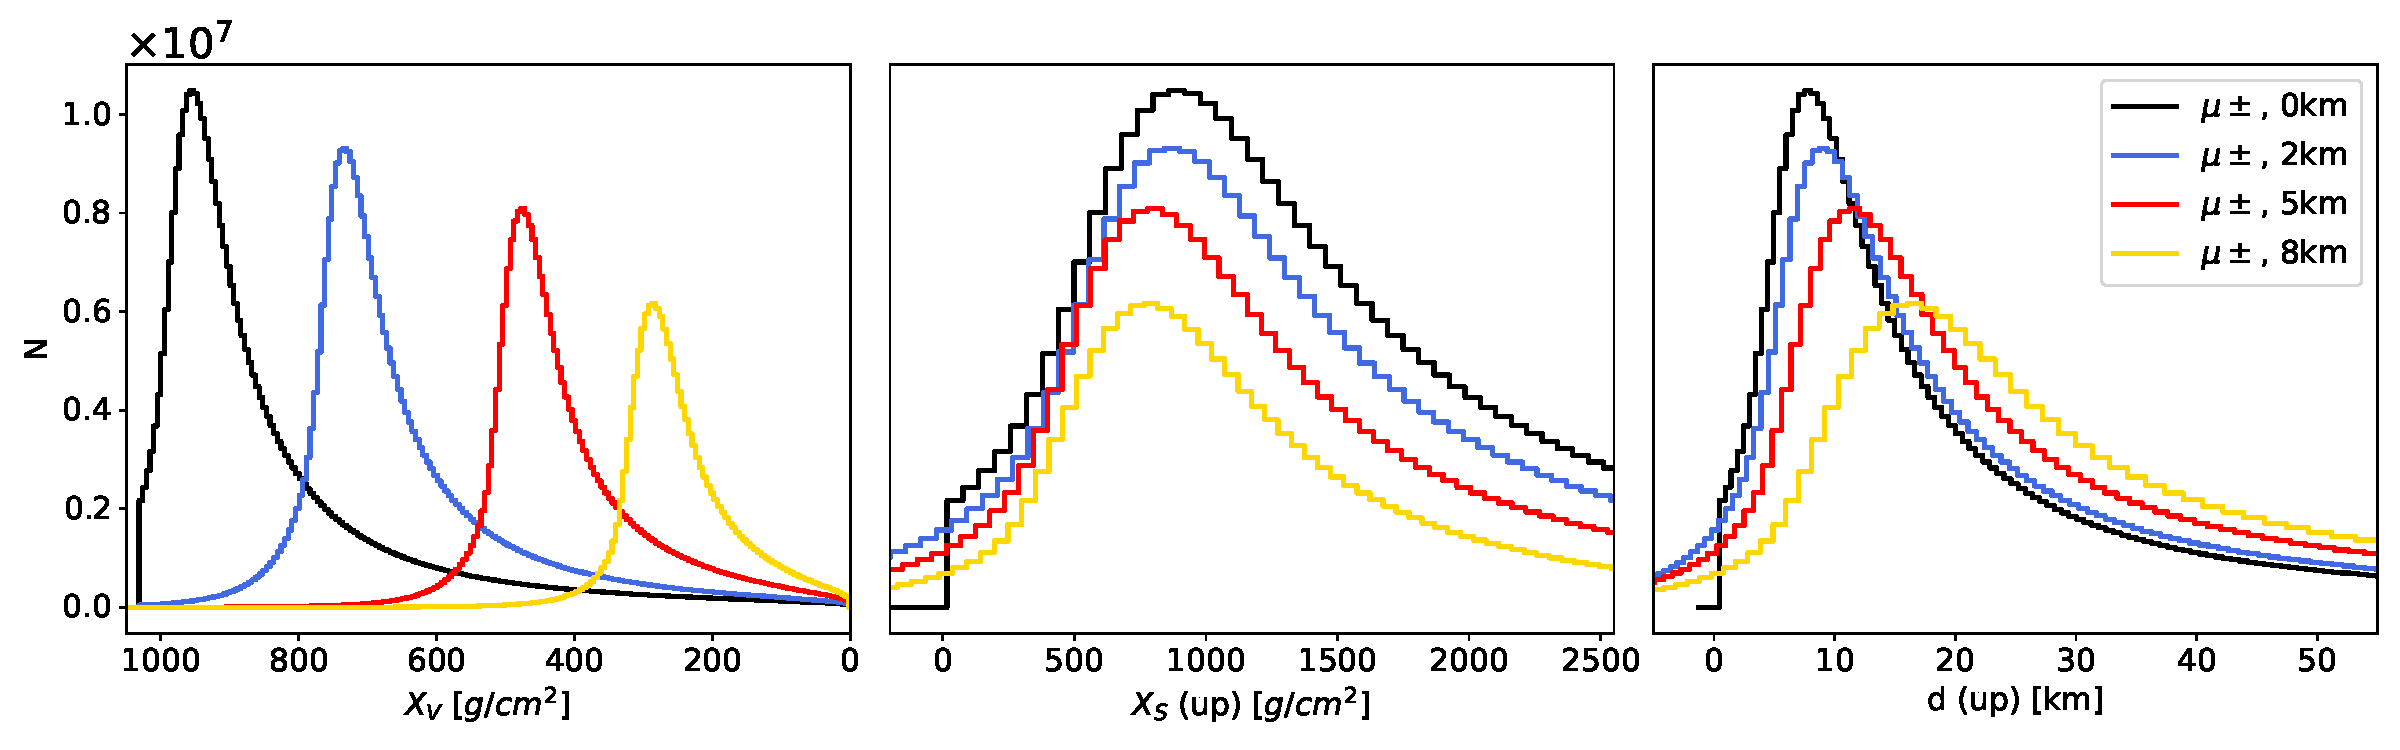
\includegraphics[width=.95\linewidth]{figures/cascadas/upgoing_p_1EeV_95deg_varh_mu_v2}
\end{figure}
\end{frame}
\begin{frame}[noframenumbering]{Aux.: Desintegración de muones en cascadas hacia arriba}
	\begin{columns}
		\column{.45\textwidth}
		\begin{figure}[H]
			\centering
			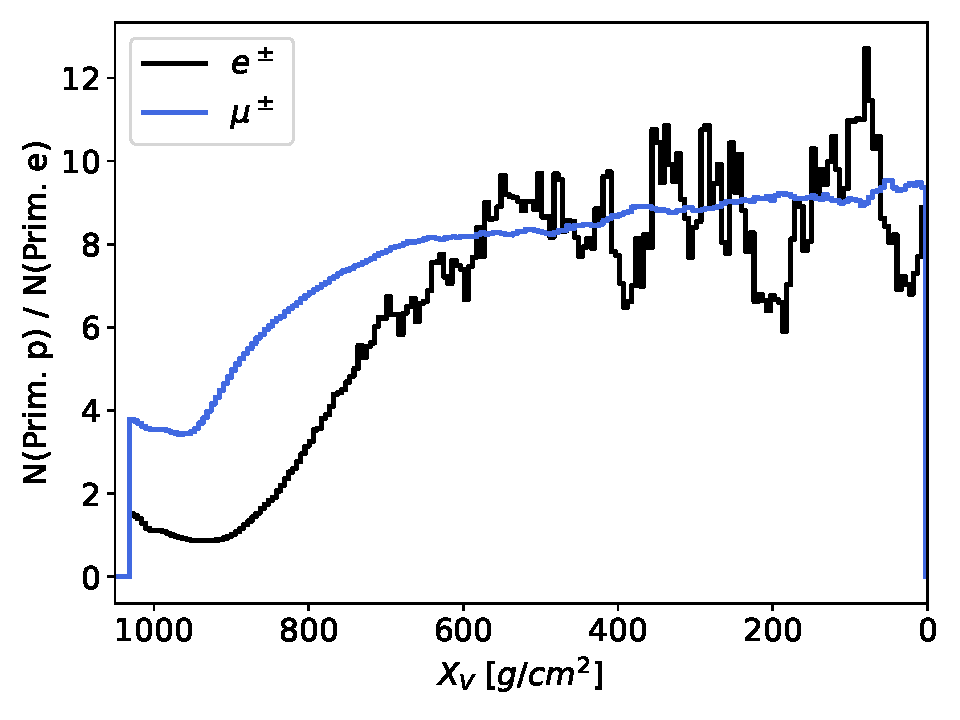
\includegraphics[width=1\linewidth]{figures/cascadas/frac_emu_Primpe}
		\end{figure}
		\column{.45\textwidth}
		\begin{figure}[H]
			\centering
			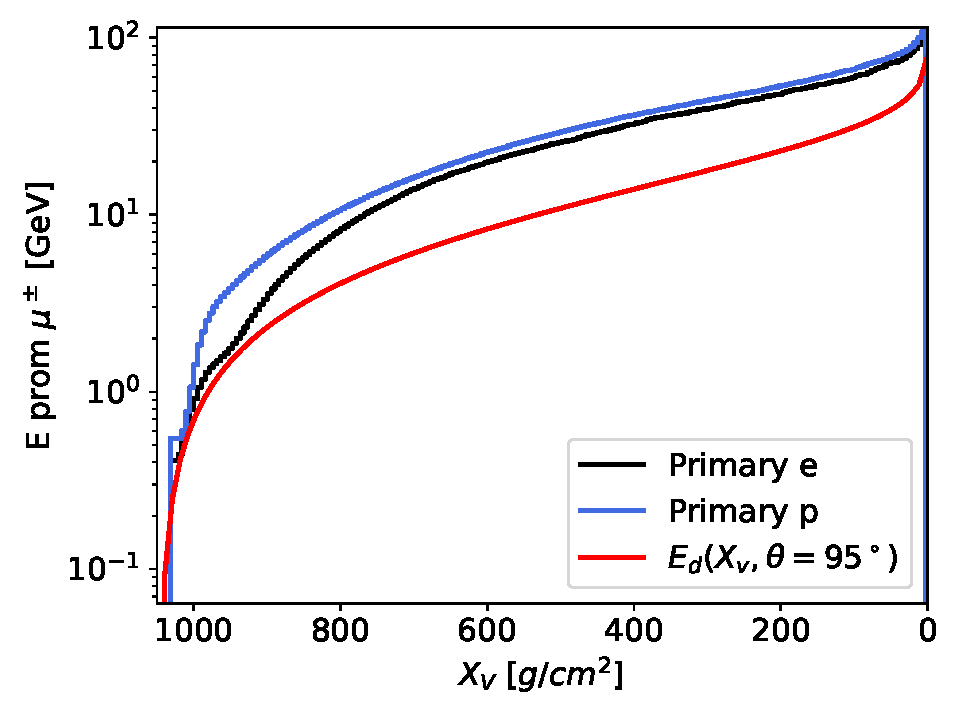
\includegraphics[width=1\linewidth]{figures/cascadas/evol_Emu_Primpe}
		\end{figure}
	\end{columns}
\end{frame}
\begin{frame}[noframenumbering]{Aux.: Energía por partícula en cascadas hacia arriba-abajo}
			\begin{figure}[H]
		\centering
		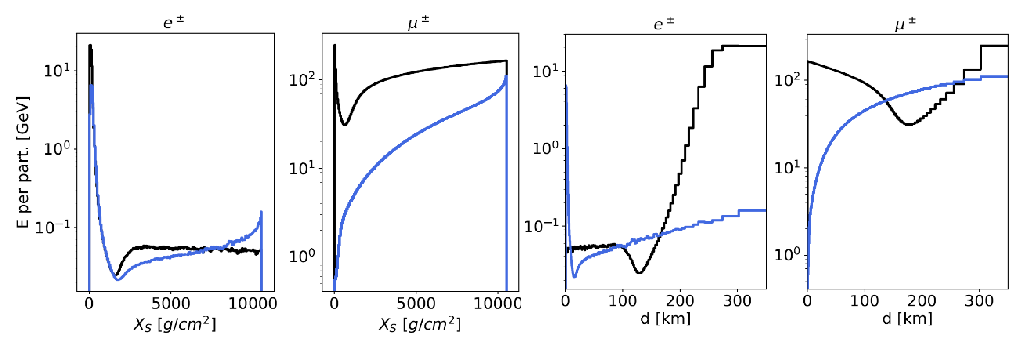
\includegraphics[width=1\linewidth]{figures/Egyperpartugdg_slides}
	\end{figure}
\end{frame}
\begin{frame}[noframenumbering]{Aux.: Fórmulas ZHS}
	$$	\vect{J}_\perp\left(\vect{r'}, t'\right)=q\vect{v}_\perp \,\delta^{(3)}\left(\vect{r}'-\vect{r}_0-\vect{v}t'\right)\left[\Theta\left(t'-t_1\right)-\Theta\left(t'-t_2\right)\right]\;,$$
	
	\footnotesize
	$$	\vect{A}\left(\vect{r}, t\right)\approx\frac{\mu q}{4\pi R}\vect{v}_\perp\frac{\Theta\left[t-nR/c-\left(1-n\beta\cos{\theta}\right)t_1\right]-\Theta\left[t-nR/c-\left(1-n\beta\cos{\theta}\right)t_2\right]}{1-n\beta\cos{\theta}}\;,$$
	
	$$\vect{E}\left(\vect{r}, t\right)\approx-\frac{\mu q}{4\pi R}\vect{v}_\perp\frac{\delta\left[t-nR/c-\left(1-n\beta\cos{\theta}\right)t_1\right]-\delta\left[t-nR/c-\left(1-n\beta\cos{\theta}\right)t_2\right]}{1-n\beta\cos{\theta}}\;,$$
	\normalsize
	
	$$\vect{E}\left(\vect{r}, \omega\right)\approx-\frac{\mu q}{2\pi R}\vect{v}_\perp \exp\left(i\omega\frac{nR}{c}\right)\frac{e^{i\omega(1-n\beta\cos{\theta})t_1}-e^{i\omega(1-n\beta\cos{\theta})t_2}}{1-n\beta\cos{\theta}}\;.$$
\end{frame}
\begin{frame}[noframenumbering]{Aux.: Señal de radio en cascada vertical hacia abajo ($E_y$)}
	\begin{columns}
		\column{.49\textwidth}
		\begin{figure}[H]
			\centering
			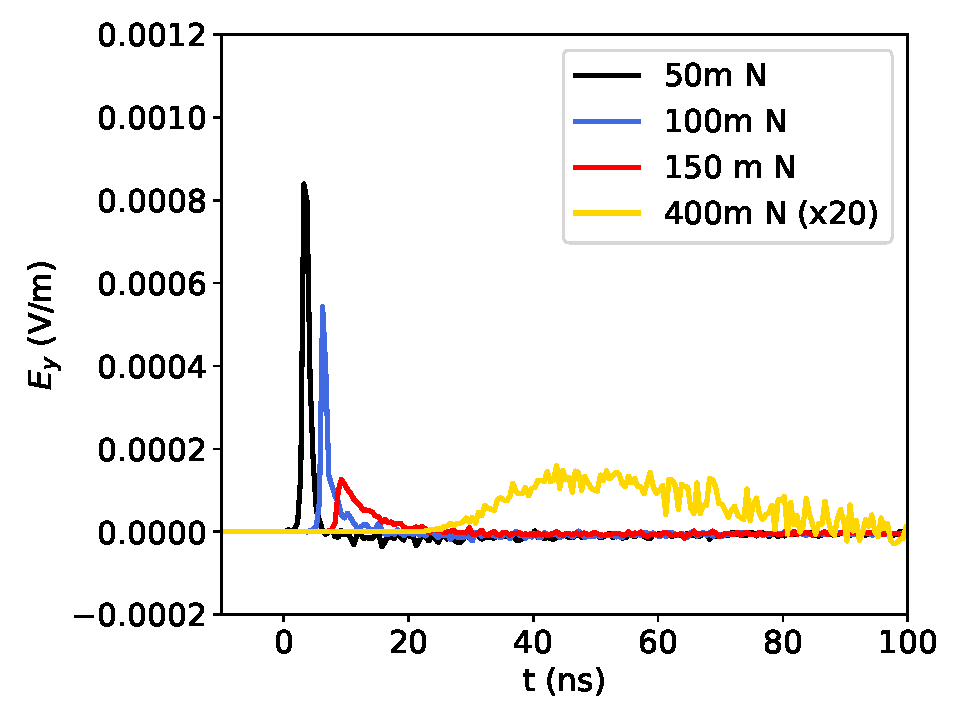
\includegraphics[width=.8\linewidth]{figures/radio/p_1e17_0deg_EW_N_v2}
		\end{figure}
			\begin{figure}[H]
		\centering
		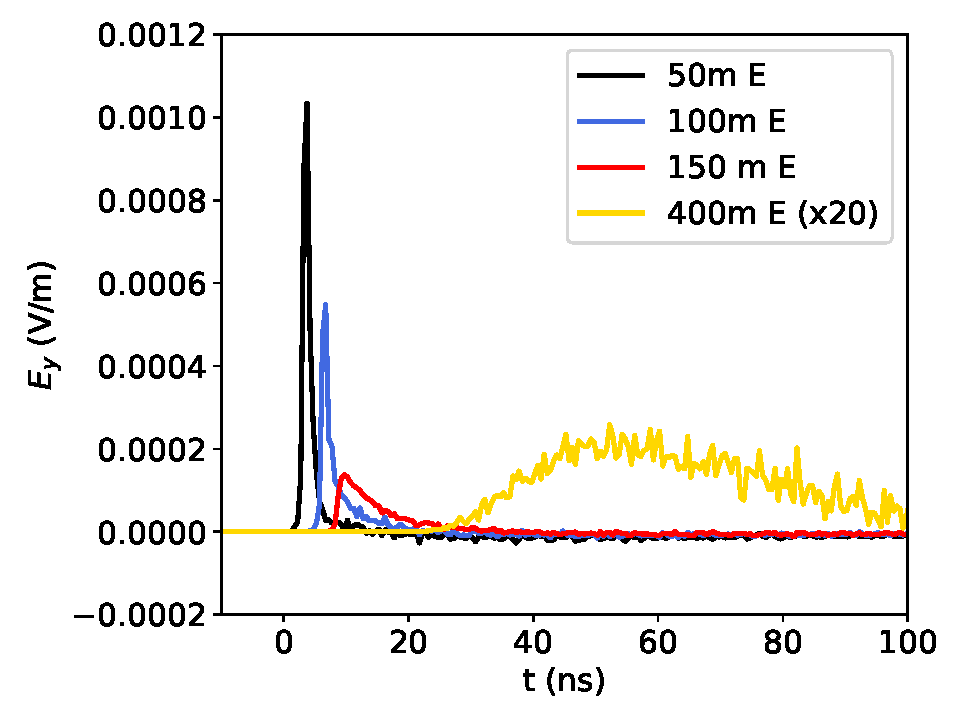
\includegraphics[width=.8\linewidth]{figures/radio/p_1e17_0deg_EW_E_v2}
	\end{figure}
		\column{.49\textwidth}
			\begin{figure}[H]
		\centering
		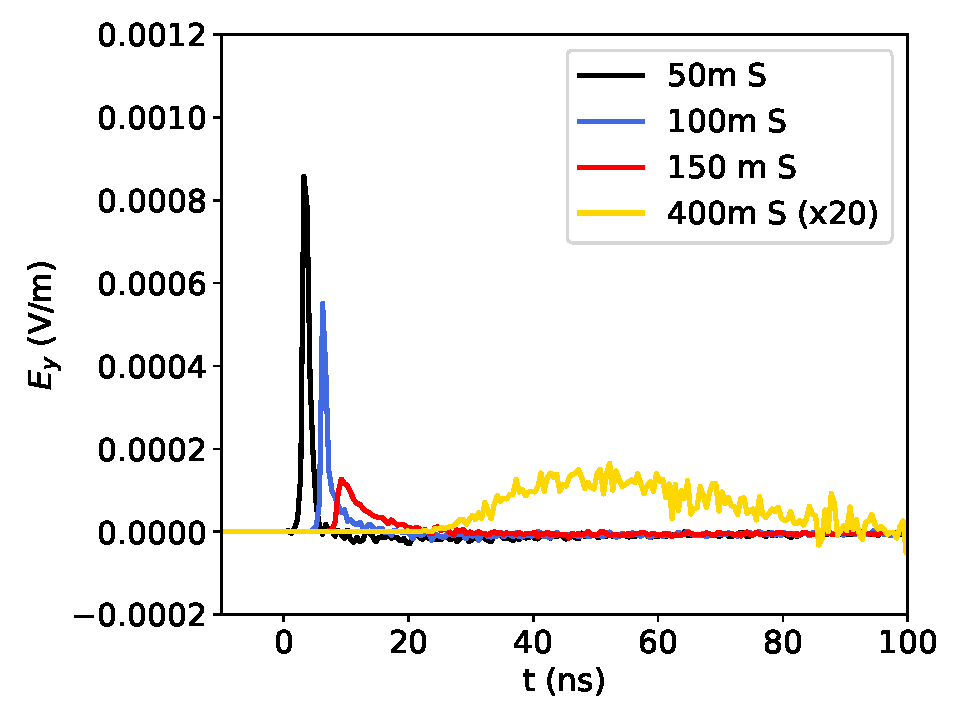
\includegraphics[width=.8\linewidth]{figures/radio/p_1e17_0deg_EW_S_v2}
	\end{figure}
	\begin{figure}[H]
		\centering
		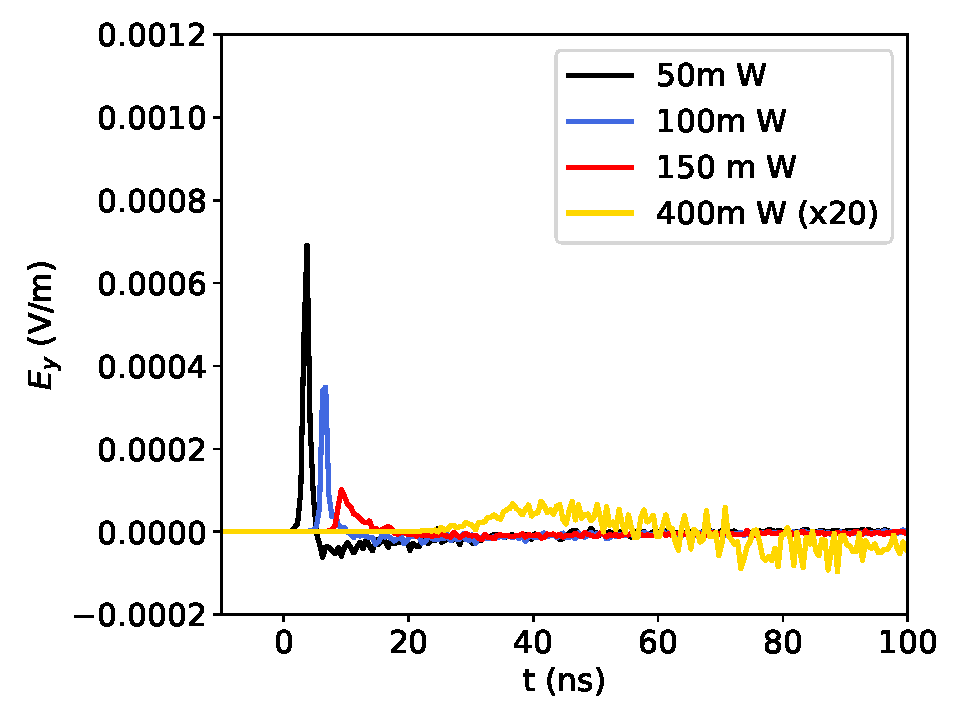
\includegraphics[width=.8\linewidth]{figures/radio/p_1e17_0deg_EW_W_v2}
	\end{figure}
	\end{columns}
\end{frame}
\begin{frame}[noframenumbering]{Aux.: Señal de radio en cascada vertical hacia abajo ($E_x$)}
		\begin{columns}
		\column{.49\textwidth}
		\begin{figure}[H]
			\centering
			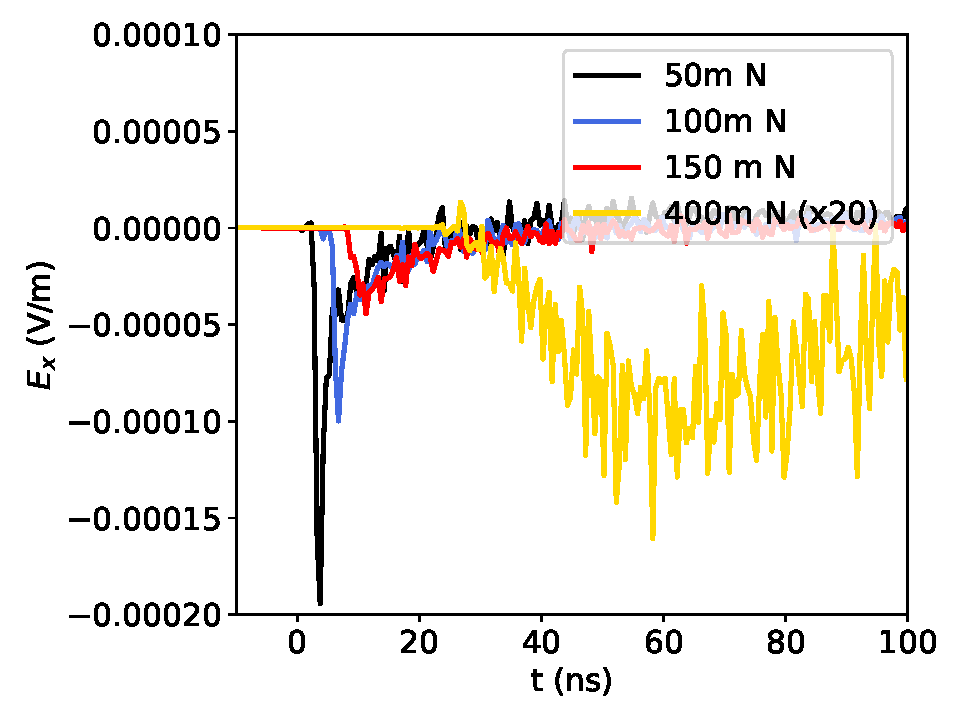
\includegraphics[width=.8\linewidth]{figures/radio/p_1e17_0deg_NS_N_v2}
		\end{figure}
		\begin{figure}[H]
			\centering
			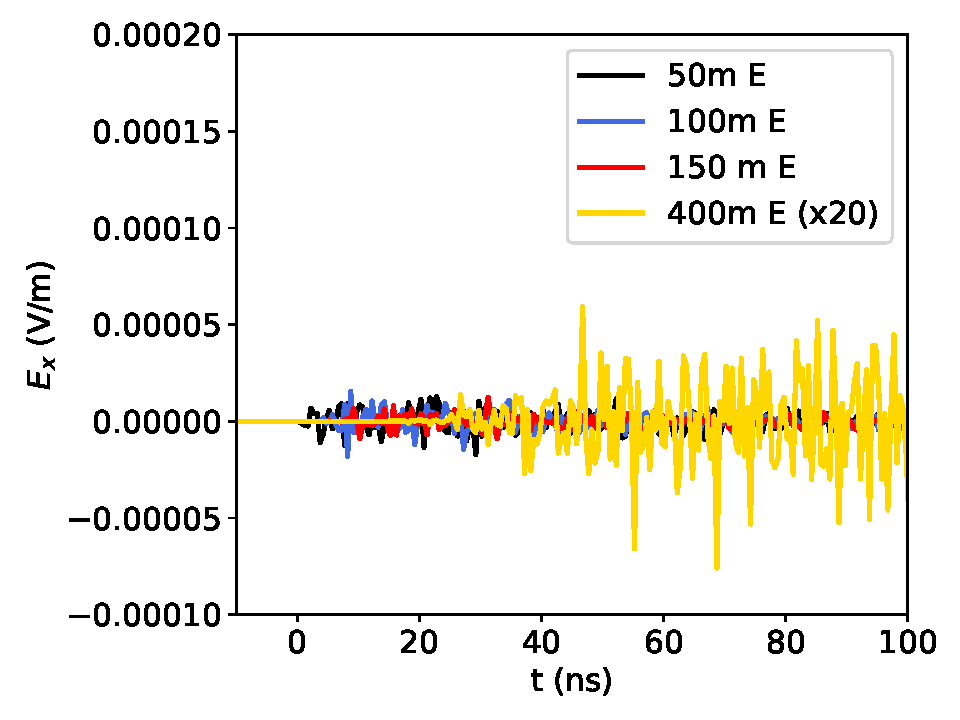
\includegraphics[width=.8\linewidth]{figures/radio/p_1e17_0deg_NS_E_v2}
		\end{figure}
		\column{.49\textwidth}
		\begin{figure}[H]
			\centering
			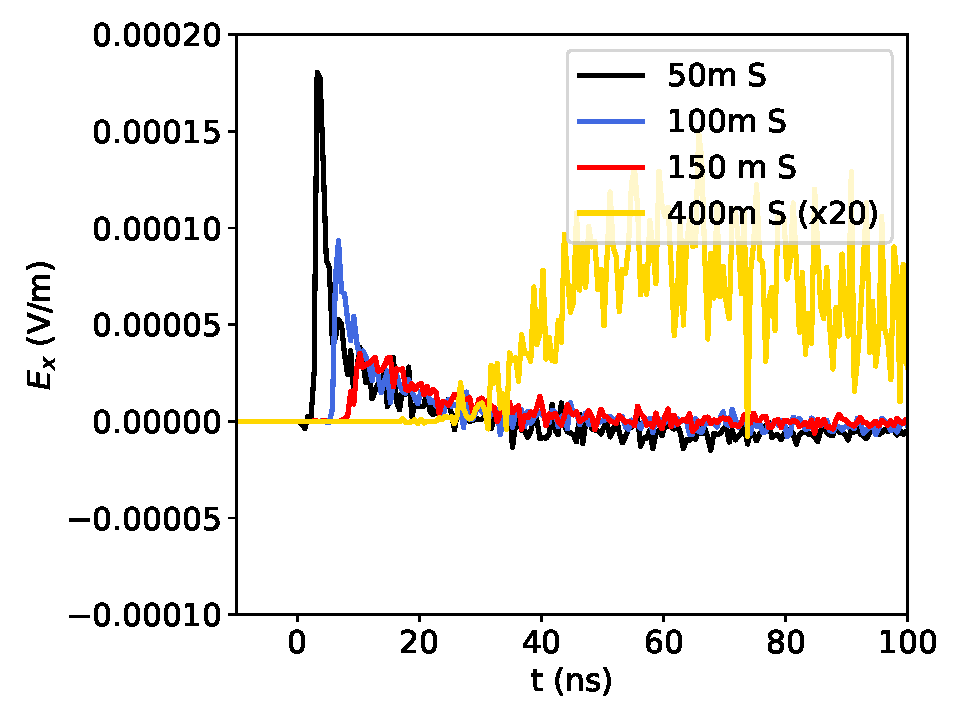
\includegraphics[width=.8\linewidth]{figures/radio/p_1e17_0deg_NS_S_v2}
		\end{figure}
		\begin{figure}[H]
			\centering
			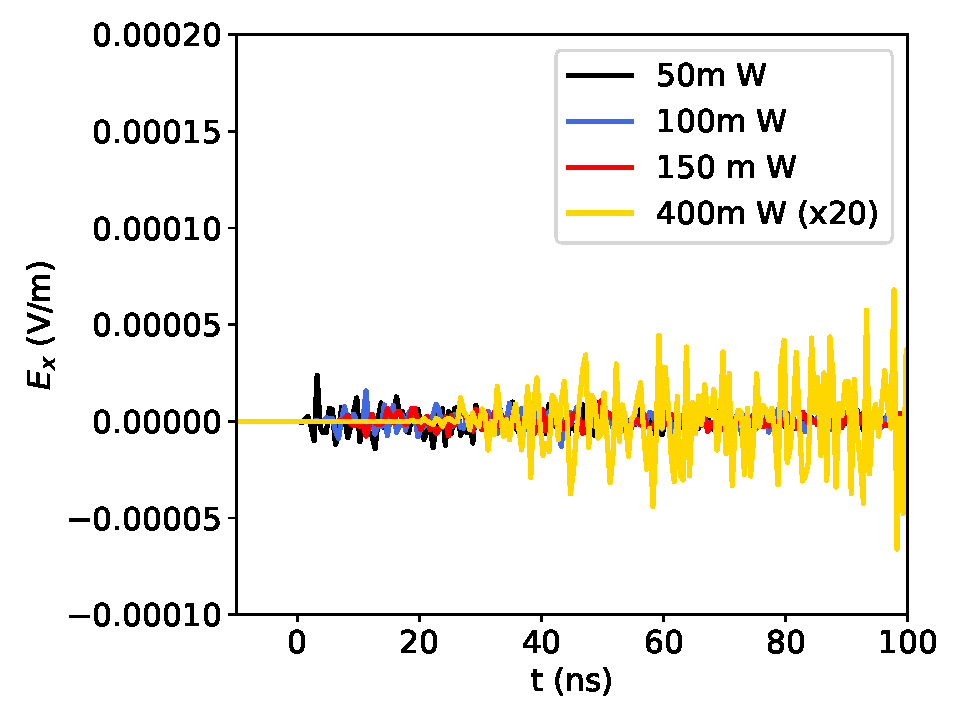
\includegraphics[width=.8\linewidth]{figures/radio/p_1e17_0deg_NS_W_v2}
		\end{figure}
	\end{columns}
\end{frame}
\begin{frame}[noframenumbering]{Aux.: Modelo geométrico para la coherencia de la señal}
	\begin{figure}[H]
		\centering
		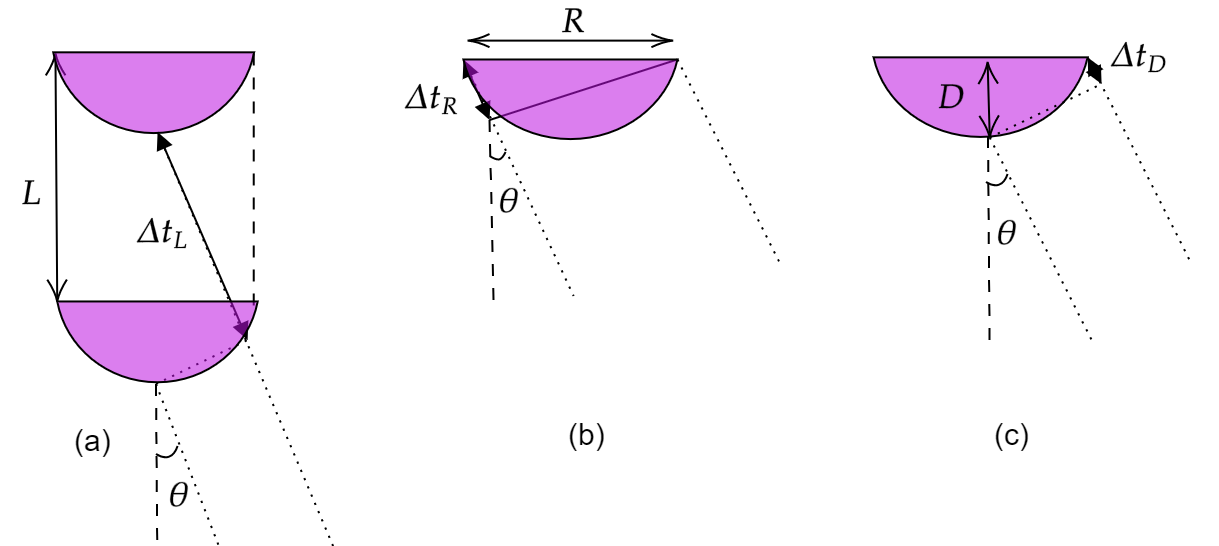
\includegraphics[width=1\linewidth]{figures/radio/coherence_v2}
	\end{figure}
\end{frame}
\end{document}